\chapter{Перехідна функція антени з круговою апертурою}
\label{ch:linear}

%%%%%%%%%%%%%%%%%%%%%%%%%%%%%%%%%%%%%%%%%%%%%%%%%%%%%%%%%%%%%%%%%%%%%%%%%%%%%%%
\section{Наближення кругової апертури}

На початку 70-их років інтерес до імпульсної радіофізики був збуджений
мілітарним застосуванням переваг надширокосмугових радарних та 
телекомунікаційних систем, як в Україні \cite{imp:Dumin1996} так 
і за кордоном \cite{imp:BaumIN0105}. Сьогодні, наробітки минулого 
століття знайшли своє застосування у системах інтернету речей, як 
наприклад Apple SoC U1 \textcolor{red}{ПОЯСНИТИ} % \cite{}.

Широким класом технічних рішень для напрямленого випромінювання 
надширокосмугового електричного струму є антени імпульсного випромінювання.
Серед них можна виділити чотири класи за способом вирівнювання фронту хвиль:
%
\begin{enumerate}
	\item Без вирівнювання сферичного фронту
	\item \textcolor{red}{Лінзові сповільнювачі}
	\item Рефлекторні антени
	\item Комбіновані архітектури \cite{imp:BaumSSN0379}
\end{enumerate}

Живлення такого класу антен зазвичай виконується ТЕМ рупором, що під'єднується 
до коаксіального кабелю через балун. Кожен з перелічних типів антен має свої
переваги, недоліки та сферу застосування. Даний розділ присвячується 
дослідженню саме лінзових антен імпульсного випромінювання (LIRA). 

Антени типу LIRA мають численні переваги над рефлекторними. Перш за все це
більш високий коефіцієнт підсилення антени \cite{imp:BaumUWBSP1}. По-друге,
лінзові антени не мають області тіні від опромінювача та краще узгоджуються
на практиці \cite{imp:BaumSSN0377}. Також експериментальне порівняння LIRA 
та RIRA показують меншої тривалості. З недоліків варто відзначити важкість 
виготовлення лінз точної форми та вагу антени.

Розглянемо задачу збудження такої антени нестаціонарним імпульсним струмом,
деякої часової залежності $ f(t) $, з умовою існування першої та другої 
похідної. Ефективна тривалість перехідного процесу $ f(t) $ за метрикою FWHM 
розглядається в межах від десятків пікосекунд до декількох наносекунд.

Сферична хвиля проходить крізь систему діелектричних лінз розташованих у 
розкриві формуючи квазі-одномоментне збудження плаского фронту у розкриві. 
Формою розкриву зазвичай вибирають кругову апертуру. Таким чином, у першому 
наближенні, у розкриві формується рівномірно розподілений сторонній плаский 
електричний струм напрямлений від одного плеча рупора до іншого. Вперше така
апроксимація була запропонована 1985 р. \cite{imp:Wu1985} та 
емпірично перевірена 1991 р. \cite{imp:Wu1991}.

Серед лінзового класу антен, що формують розподіл стороннього струму у вигляді 
плаского диску варто відзначити антену Рис.~\ref{fig:lira_baum}, що спершу
представив Ву \cite{imp:Wu1987}, а згодом і Баум \cite{imp:BaumSSN0377}. 
Лінза антени виконана у формі витягнутого сфероїда, а розкрив ТЕМ рупора 
цілком заповнено діелектриком. Таким чином мінімізується відбиття. 
Скруглений рупор починається в одному фокусі еліпсоїда, а закінчується в 
другому, таким чином радіус розкриву є фокальним параметром еліпсоїда.
В якості матеріалу для лінзи пропонується використовувати поліетилен 
високої густини ($\epsilon = 2.3 $).

\begin{figure}[htbp] \begin{center}
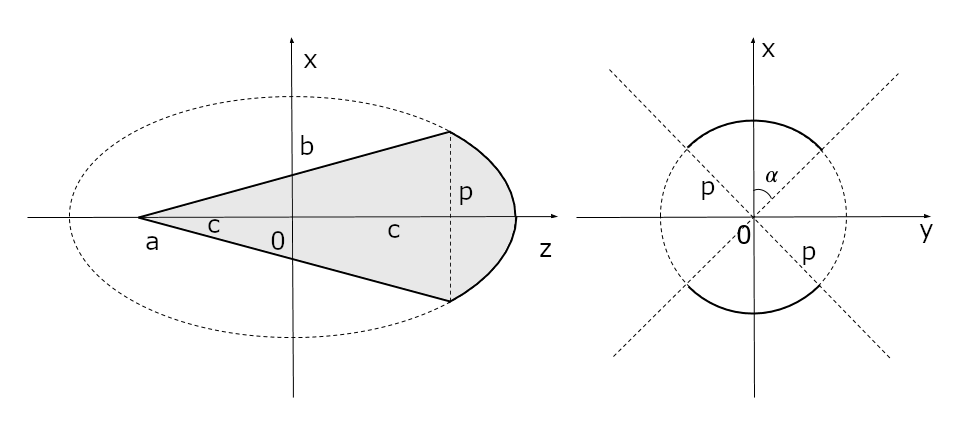
\includegraphics[scale=0.5]{Baum_LIRA}
\caption{Геометрія лінзевої антени Баума та Ву} \label{fig:lira_baum}
\end{center} \end{figure}

В 1991 р. Ву представив антену, що краще підходить під наближення  
плаского диску електричного струму \cite{imp:Wu1991}. Гіперболічна лінза 
забезпечує розташування площини рівних фаз в самому розкриві, що і утворює
плаский диск \ref{fig:lira_wu}. Цікавою варіацією цієї антени є заміна 
діелектричного наповнення $ \epsilon_1 $ та лінзи $ \epsilon_2 $ на матеріал,
діелектрична характеристика якого є функцією координат $ \epsilon(\rho, z) $.
Таким чином відбиття від внутрішньої поверхні лінзи зникне і характеристики 
антени покращаться. Важливим мінусом такої архітектурне стає важкість 
виготовлення лінзи.

\begin{figure}[htbp] \begin{center}
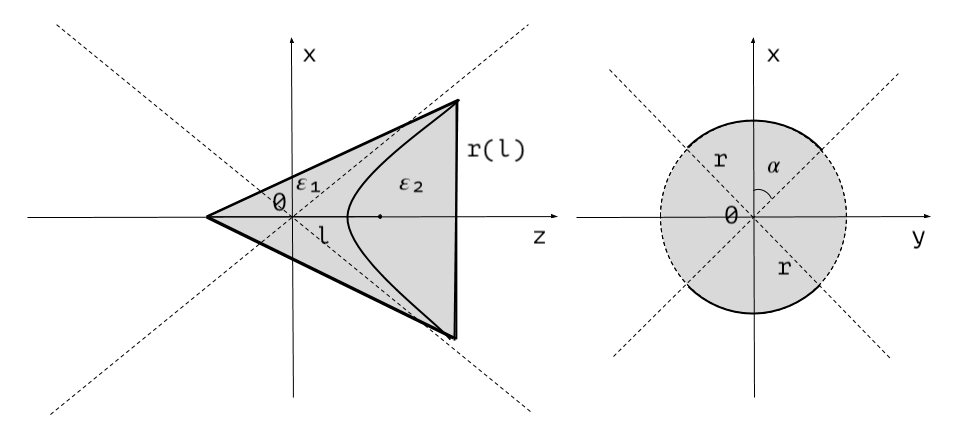
\includegraphics[scale=0.5]{Wu_LIRA}
\caption{Геометрія лінзової антени Ву} \label{fig:lira_wu}
\end{center} \end{figure}

Прямим призначенням таких антен є телекомунікація, радіолокація і лабораторні 
вимірювання. Проте цікавість таких антен пояснюється ще і аномально повільним
згасанням енергії імпульсного поля з відстанню, що було теоретично 
передбачено \cite{imp:Wu1987}. Цей ефект відомий за назвою електромагнітний 
снаряд.

Фізична модель плаского диску описує поле LIRA лише у першому наближенні.
Така модель не враховує вихровий магнітний сторонній струм, що існує на ряду 
з пласким електричним, а також не враховує струми що течуть назад в генератор 
відбившись від краю рупора - поле такого струму залишає довгий "хвіст" після 
основного імпульсу. Проте емпіричне дослідженнях 
\cite{imp:BaumSSN0396,imp:BaumSSN0401} показує, що при належному 
узгодженні, паразитний вплив відбиття фактично відсутній, а перехідна 
функція отримана експериментальним шляхом відповідає розв'язку, що дає 
плаский диск.

Розв'язок задачі плаского диску шукали різними методами. Першими були 
отримані наближені розв'язки в частотній області 
\cite{imp:Wu1985,imp:Sodin1992-10}. Також, розв'язок для цієї задачі знайдено 
у часовій області \cite{imp:Dumin1996}. Недоліком наявних розв'язків є те,
що вони не надають часову залежіть напруженості поля в довільних точках 
спостереження в явному виді. При самоїді поля крізь середовище на значення 
напруженості поля в кожній точці спостереження та в будь-який момент вплавить
всі пов'язані зі спостереженням події. Таким чином наявність розв'язання в 
будь-якій точці спостереження - необхідна умова.
%
%%%%%%%%%%%%%%%%%%%%%%%%%%%%%%%%%%%%%%%%%%%%%%%%%%%%%%%%%%%%%%%%%%%%%%%%%%%%%%%
\section{Розв'язання методом еволюційних рівнянь} \label{sec:tranc_resp}
%
Розглянемо сторонній електричний нестаціонарний струм $ \vect{j_0} (r,t) $ 
в якості єдиного джерела електромагнітного поля. Нехай, струм 
одно-напрямлений, рівномірно-розподілений та має форму плаского диску 
нульової товщини. Для розв'язання прямої задачі електродинаміки для 
довільної часової $ f(t) $ залежності нестаціонарного струму 
$ \vect{j_0} (r,t) $, достатньо отримати розв'язок для перехідної функції, 
тобто $ f(t) = H(t) $, де $ H(t) $ - функція Хевісайда. Тоді, математично 
його можна описати в циліндричних координатах $ \rho, \varphi, z $, як
%
\begin{equation}
\vect{j_0} \left( r, t \right) = \vect{J} = \vect{x_0} A_0 H(t) \delta(z) 
\left(  H(\rho) - H(\rho - R) \right),
\end{equation}
%
де $ A_0 $ - максимальна амплітуда струму, $ R $ - радіус диску,
$ \delta(z) $ - символ Кронекера, а 
$ \vect{x_0} = \vect{\rho_0} \cos \varphi - \vect{\varphi_0} \sin \varphi $ 
- декартовий орт OX. 
%
\begin{figure}[htbp] \begin{center}
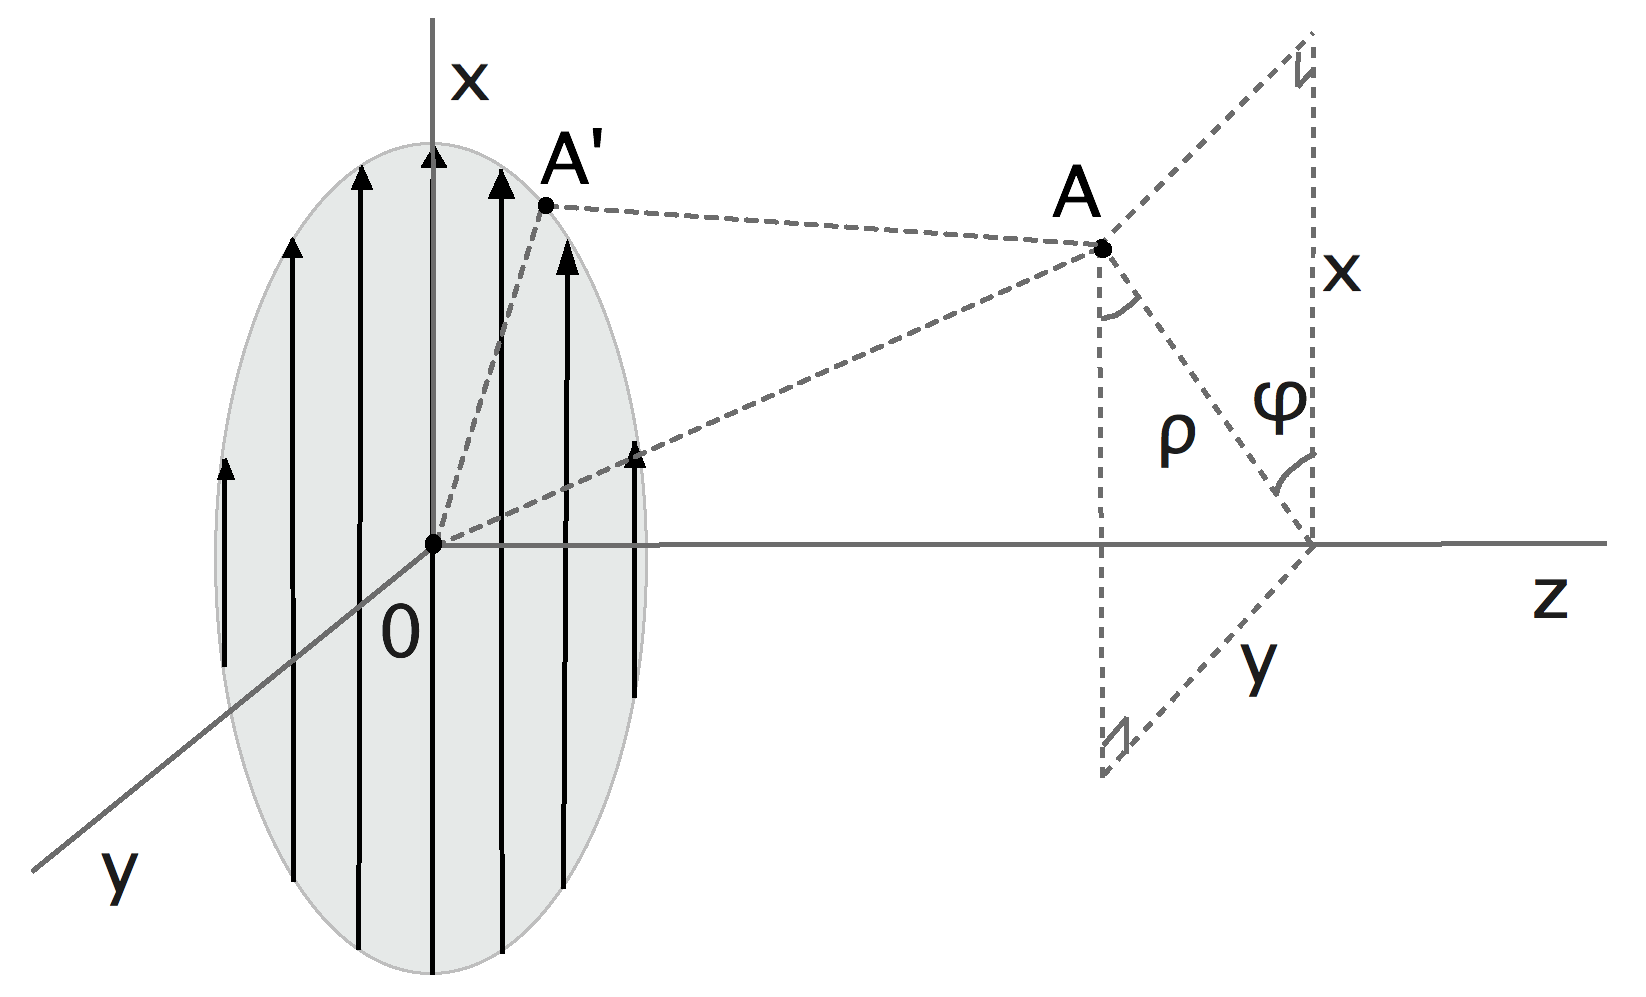
\includegraphics[scale=0.55]{PlaneDisk}
\caption{Геометрія випромінювача} \label{fig:pdisk}
\end{center} \end{figure}
%
\textcolor{blue} { \begin{equation*} \begin{aligned}
\begin{cases}
\vect{\rho_0} = \vect{x_0} \cos \varphi + \vect{y_0} \sin \varphi \\
\vect{\varphi_0} = - \vect{x_0} \sin \varphi + \vect{y_0} \cos \varphi
\end{cases} \Rightarrow \mathbf{A} = \left( \begin{array}{cc}
\cos \varphi & \sin \varphi \\
- \sin \varphi & \cos \varphi
\end{array} \right)
\end{aligned} \end{equation*} }
%
\textcolor{blue} { \begin{equation*} \begin{aligned}
\vect{j_0} \left( \vect{\rho_0}, \vect{\varphi_0} \right) = 
\mathbf{A} \vect{j_0} \left( \vect{x_0}, \vect{y_0} \right) = \\
= H(t) \delta(z) (  H(\rho) - H(\rho - R) ) 
( \vect{\rho_0} \cos \varphi - \vect{\varphi_0} \sin \varphi )
\end{aligned} \end{equation*} }
%
Для застосування методу еволюційних рівнянь знайдемо модовий розклад 
струму
%
\begin{equation} \label{eq:jm_base}
j_m \left( r, t; \nu \right) = \frac{\sqrt{\mu_0}}{2\pi} 
\int \limits_{0}^{2\pi} d \varphi \int \limits_{0}^{\infty} \rho d \rho 
\vect{j_0} \crossprod{ \nabla_\perp \Psi_m^* }{ \vect{z_0} },
\end{equation}
%
де $ \Psi_m^* $ - комплексно спряжена базисна функція \cite{imp:Dumin2010}.
%
\textcolor{blue} { \begin{equation*} \begin{aligned}
\crossprod{ \nabla_\perp \Psi_m^* }{ \vect{z_0} } = 
- \sqrt{\nu} e^{-im\varphi} \left( 
\vect{\varphi_0} \frac{J_{m-1} (\nu \rho) - J_{m+1} (\nu \rho)}{2} + 
\right. \\ + \left. i m \vect{\rho_0} \frac{J_m (\nu \rho)}
{\rho \nu} \right) = - \sqrt{\nu} e^{-im\varphi} \left( 
\vect{\varphi_0} \frac{J_{m-1} (\nu \rho) - J_{m+1} (\nu \rho)}{2} + 
\right. \\ + \left. i \vect{\rho_0} \frac{J_{m-1} (\nu \rho) + 
J_{m+1} (\nu \rho)}{2} \right)
\end{aligned} \end{equation*} }
%
\textcolor{blue} { \begin{equation*} \begin{aligned}
\vect{j_0} \crossprod{ \nabla_\perp \Psi_m^* }{ \vect{z_0} } = 
- \sqrt{\nu} ( \cos m \varphi - i \sin m \varphi ) 
H(t) \delta(z) ( H(\rho) - H(\rho - R) ) \cdot \\ \cdot \left( 
i \frac{J_{m-1} (\nu \rho) + J_{m+1} (\nu \rho)}{2} \cos \varphi
- \frac{J_{m-1} (\nu \rho) - J_{m+1} (\nu \rho)}{2} \sin \varphi
\right)
\end{aligned} \end{equation*} }
%
\textcolor{blue} { \begin{equation*} \begin{aligned}
j_m = \frac{\sqrt{\mu_0}}{2\pi} \sqrt{\nu} \delta(z) H(t) \cdot \\
\cdot \Big( \int \limits_{0}^{2\pi} d \varphi \sin \varphi 
( \cos m \varphi - i \sin m \varphi) \int \limits_{0}^{R} 
\frac{J_{m-1} (\nu \rho) - J_{m+1} (\nu \rho)}{2} \rho d \rho - \\
- i \int \limits_{0}^{2\pi} d \varphi \cos \varphi 
( \cos m \varphi - i \sin m \varphi) \int \limits_{0}^{R} 
\frac{J_{m-1} (\nu \rho) + J_{m+1} (\nu \rho)}{2} \rho d \rho \Big)
\end{aligned} \end{equation*} }
%
\textcolor{blue} { \begin{equation*} \begin{aligned}
j_m = \frac{\sqrt{\mu_0}}{2\pi} \sqrt{\nu} \delta(z) H(t) 
i\pi ( \delta_{m,-1} - \delta_{m,1} ) \int \limits_{0}^{R} 
\frac{J_{m-1} (\nu \rho) - J_{m+1} (\nu \rho)}{2} \rho d \rho - \\
- \frac{\sqrt{\mu_0}}{2\pi} \sqrt{\nu} \delta(z) H(t) 
i\pi ( \delta_{m,-1} + \delta_{m,1} ) \int \limits_{0}^{R} 
\frac{J_{m-1} (\nu \rho) + J_{m+1} (\nu \rho)}{2} \rho d \rho =
\end{aligned} \end{equation*} }
%
\textcolor{blue} { \begin{equation*} \begin{aligned}
= i \frac{\sqrt{\mu_0 \nu}}{4} \delta(z) H(t)
\delta_{m,-1} \int \limits_{0}^{R} \left( J_{-2} (\nu \rho) - 
J_0 (\nu \rho) \right) \rho d \rho - \\
- i \frac{\sqrt{\mu_0 \nu}}{4} \delta(z) H(t)
\delta_{m,1} \int \limits_{0}^{R} \left( J_{0} (\nu \rho) - 
J_2 (\nu \rho) \right) \rho d \rho - \\
- i \frac{\sqrt{\mu_0 \nu}}{4} \delta(z) H(t)
\delta_{m,-1} \int \limits_{0}^{R} \left( J_{-2} (\nu \rho) +  
J_0 (\nu \rho) \right) \rho d \rho - \\
- i \frac{\sqrt{\mu_0 \nu}}{4} \delta(z) H(t)
\delta_{m,1} \int \limits_{0}^{R} \left( J_{0} (\nu \rho) +
J_2 (\nu \rho) \right) \rho d \rho =
\end{aligned} \end{equation*} }
%
\textcolor{blue} { \begin{equation*} \begin{aligned}
= - i \frac{\sqrt{\mu_0 \nu}}{2} \delta(z) H(t) 
(\delta_{m,1} + \delta_{m,-1}) 
\int \limits_{0}^{R} \left( J_{0} (\nu \rho) + 
J_2 (\nu \rho) \right) \rho d \rho - \\
- i \frac{\sqrt{\mu_0 \nu}}{2} \delta(z) H(t) 
(\delta_{m,1} + \delta_{m,-1}) 
\int \limits_{0}^{R} \left( J_{0} (\nu \rho) -
J_2 (\nu \rho) \right) \rho d \rho = \\
= - i \frac{\sqrt{\mu_0 \nu}}{2} \delta(z) H(t) 
(\delta_{m,1} + \delta_{m,-1}) 
\int \limits_{0}^{R} J_{0} (\nu \rho) \rho d \rho
\end{aligned} \end{equation*} }
%
\textcolor{blue} { \begin{equation*} \begin{aligned}
\int \limits_{0}^{R} J_{0} (\nu \rho) \rho d \rho = 
\frac{1}{\nu^2} \int \limits_{0}^{R} J_{0} (\nu \rho) \nu \rho d \nu \rho =
\left. \frac{\rho J_1 (\nu \rho) }{\nu} \right|_{0}^{R} = 
\frac{R J_1 (\nu R)}{\nu}
\end{aligned} \end{equation*} }
%
Після інтегрування $ \eqref{eq:jm_base} $ отримаємо тільки дві не нульові 
рівні моди, визначені через символи Кронекера $ \delta_{m,\pm1} $.
%
\begin{equation} 
j_m (z, t; \nu) = - i R A_0 \frac{\sqrt{\mu_0}}{2} \delta(z) H(t) 
\frac{\delta_{m,1} + \delta_{m,-1}}{\sqrt{\nu}} J_1 (\nu R)
\end{equation}
%
Тепер знайдемо поздовжні модові коефіцієнти $ h_1 $ та $ h_{-1} $ 
розв'язанням рівнянь Клейна-Гордона
%
\textcolor{blue} { \begin{equation*} \begin{aligned}
- \epsilon \partial_{ct} (V_m^h) - \partial_z I_m^h + \nu^2 h_m = 
\frac{\sqrt{\mu_0}}{2 \pi} \int_0^{2\pi} d \varphi 
\int_0^{\infty} \rho d \rho \crossprod{\vect{z_0}}{\vect{J_\perp}}
\nabla_\perp \Psi_m^* (\nu) 
\end{aligned} \end{equation*} }
%
\textcolor{blue} { \begin{equation*} \begin{aligned}
\crossprod{\vect{z_0}}{\vect{J_\perp}} \nabla_\perp \Psi_m^* (\nu) =
\vect{J_\perp} \crossprod{\nabla_\perp \Psi_m^* (\nu)}{\vect{z_0}}
\end{aligned} \end{equation*} }
%
\textcolor{blue} { \begin{equation*} \begin{aligned}
\epsilon \partial_{ct} \left( \mu \partial_{ct} h_m \right) -
\mu^{-1} \partial_z \left( \mu  \partial_z h_m \right) + 
\nu^2 h_m = j_m (z,t,\nu)
\end{aligned} \end{equation*} }
%
\begin{equation} \begin{aligned} \label{eq:klein_gordon}
\frac{\epsilon \mu}{c^2} \frac{\partial^2 h_m}{\partial t^2} - 
\frac{\partial^2 h_m}{\partial z^2} + \nu^2 h_m = j_m (z,t,\nu).
\end{aligned} \end{equation}
%
Рівняння \eqref{eq:klein_gordon} було отримано з припущенням, що середовище 
в якому розповсюджується поле однорідне, стаціонарне та характеризуватися 
відносною діелектричною $ \epsilon $ та магнітною $ \mu $ проникненнями.
Буде зручно позначити швидкість світла в цьому середовищі за 
$ \mathit{v} = \frac{c}{\sqrt{\epsilon \mu}} $. Рівняння Клейна-Гордона
має відомий розв'язок через функцію Рімана:
%
\begin{equation} \label{eq:klein_gordon_sol}
h_m (z, t; \nu) = \iint_S j_m (t',z') G(t,t',z,z') dt' dz',
\end{equation}
%
де $ G(t,t',z,z') $ функція Рімана 
%
\begin{equation*}
G = \frac{\mathit{v}}{2} H \left( \mathit{v} (t-t') - (z-z') \right)
J_0 \left( \nu \sqrt{\mathit{v}^2 (t-t')^2 - (z-z')^2} \right).
\end{equation*}
%
З вигляду розв'язку \eqref{eq:klein_gordon_sol} можна зробити висновок, що
функція Рімана $ G(t,t',z,z') $ - це аналог функції Гріна в часовому просторі,
а тобто розв'язок рівняння Клейна-Гордона є еквівалентом принципу суперпозиції
сферичних нестаціонарних хвиль, що випромінюються кожною з точок джерела у
деякій точці спостереження у визначений час.
%
\textcolor{blue} { \begin{equation*} \begin{aligned}
h_m (z, t; \nu) = - i \mathit{V} R \frac{\sqrt{\mu_0}}{4} 
\frac{\delta_{m,1} + \delta_{m,-1}}{\sqrt{\nu}} J_1 (\nu R)
\int \limits_{0}^{\infty} \delta(z) \cdot \\ \cdot
\int \limits_{t - \frac{z}{\mathit{V}}}^{0} 
J_0 \left( \nu \sqrt{\mathit{V}^2 (t-t')^2 - (z-z')^2} \right) dt' dz' = 
i \mathit{V} R \frac{\sqrt{\mu_0}}{4} 
\frac{\delta_{m,1} + \delta_{m,-1}}{\sqrt{\nu}} J_1 (\nu R)
\cdot \\ \cdot \int \limits_{0}^{\infty} \delta(z)
\int \limits_{0}^{t - \frac{z}{\mathit{V}}} 
J_0 \left( \nu \sqrt{\mathit{V}^2 (t-t')^2 - (z-z')^2} \right) dt' dz
\end{aligned} \end{equation*} }
%
\textcolor{blue} { \begin{equation*} \begin{aligned}
h_m (z, t; \nu) = i \mathit{V} R \frac{\sqrt{\mu_0}}{4} 
\frac{\delta_{m,1} + \delta_{m,-1}}{\sqrt{\nu}} J_1 (\nu R)
\int \limits_{0}^{t - \frac{z}{\mathit{V}}} 
J_0 \left( \nu \sqrt{\mathit{V}^2 (t-t')^2 - z^2} \right) dt'
\end{aligned} \end{equation*} }
%
Користуючись властивостями дельта-функції Дірака та функції Хевісайда 
запишемо поздовжні модові коефіцієнти $ h_1 $ та $ h_{-1} $ в наступному 
виді:
%
\begin{equation} \label{eq:hm_int}
h_m = \frac{i R A_0}{4} \frac{\delta_{m,1} + \delta_{m,-1}}
{\sqrt{\nu} \sqrt{\epsilon_0 \epsilon \mu}} J_1 (\nu R) 
\int \limits_{0}^{t - \frac{z}{v}} 
J_0 \left( \nu \sqrt{v^2 (t-t')^2 - z^2} \right) dt'
\end{equation} }
%
Зараз зручно перейти до отримання поперечних морових коефіцієнтів.
Для отримання виразу для $ V_m^h = - \frac{\mu}{c} \partder{h_m}{t} $
необов'язково брати інтеграл в $ h_m $ спробуємо спростити вираз 
скориставшись залежністю через похідну по часу, тобто застосуємо 
правило ітерування Лейбніца \cite{imp:Flanders1973}, помітивши, що
%
\begin{equation*} \begin{aligned}
\partder{}{t'} J_0 \left( \nu \sqrt{v^2 (t-t')^2 - z} \right) =
- \partder{}{t} J_0 \left( \nu \sqrt{v^2 (t-t')^2 - z} \right) 
\end{aligned} \end{equation*}
%
отримаємо
%
\textcolor{blue} { \begin{equation*} \begin{aligned}
\partder{}{\theta} \int_{a(\theta)}^{b(\theta)} f(x,\theta) dx = 
\int_{a(\theta)}^{b(\theta)} \partder{f}{\theta} dx + 
f\big( b(\theta), \theta \big) \partder{b}{\theta} -
f\big( a(\theta), \theta \big) \partder{a}{\theta}
\end{aligned} \end{equation*} }
%
\textcolor{blue} { \begin{equation*} \begin{aligned}
\partder{}{t} J_0 \left( \nu \sqrt{v^2 (t-t')^2 - z} \right) = 
- \nu J_1 \left( \nu \sqrt{v^2 (t-t')^2 - z} \right) 
\partder{}{t} \sqrt{v^2 (t-t')^2 - z} = \\
-  J_1 \left( \nu \sqrt{v^2 (t-t')^2 - z} \right)
\frac{2 \nu v^2 (t-t')}{2 \sqrt{v^2 (t-t')^2 - z}} = - \nu v^2 (t-t') 
\frac{J_1 \left( \nu \sqrt{v^2 (t-t')^2 - z} \right)}
     {\sqrt{v^2 (t-t')^2 - z}}
\end{aligned} \end{equation*} }
%
\textcolor{blue} { \begin{equation*} \begin{aligned}
\partder{}{t} \int \limits_{0}^{t - \frac{z}{v}} 
J_0 \left( \nu \sqrt{v^2 (t-t')^2 - z^2} \right) dt' = \\
= \int \limits_{0}^{t - \frac{z}{v}} 
\partder{}{t} J_0 \left( \nu \sqrt{v^2 (t-t')^2 - z^2} \right) dt' +
J_0 (0) - 0 \cdot \left( \nu \sqrt{v^2 (t-t')^2 - z^2} \right) = \\
= - \int \limits_{0}^{t - \frac{z}{v}} 
\partder{}{t'} J_0 \left( \nu \sqrt{v^2 (t-t')^2 - z^2} \right) dt' + 1 =
- \Big. J_0 \left( \nu \sqrt{v^2 (t-t')^2 - z^2} \right) \Big|_{0}^{t - \frac{z}{v}} + 1 = \\
- J_0 \left( \nu \sqrt{z^2 - z^2} \right) + J_0 \left( \nu \sqrt{v^2 t^2 - z^2} \right) + 1 = 
J_0 \left( \nu \sqrt{v^2 t^2 - z^2} \right)
\end{aligned} \end{equation*} }
%
\begin{equation*} \begin{aligned}
\partder{}{t} \int \limits_{0}^{t - \frac{z}{v}} 
J_0 \left( \nu \sqrt{v^2 (t-t')^2 - z^2} \right) dt' =
J_0 \left( \nu \sqrt{v^2 t^2 - z^2} \right),
\end{aligned} \end{equation*}
%
\textcolor{blue} { \begin{equation*} \begin{aligned}
V_m^h = - \frac{\mu}{c} \partder{h_m}{t} = 
\sqrt{\mu_0} \sqrt{\frac{\mu}{\epsilon}} \frac{iR A_0}{4} 
\frac{\delta_{m,1} + \delta_{m,-1}}{\sqrt{\nu}} J_1 (\nu R)
J_0 \left( \nu \sqrt{\mathit{v}^2 t^2 - z^2} \right)
\end{aligned} \end{equation*} }
%
тоді можемо записати формулу для коефіцієнтів $ V_m^h $
%
\begin{equation} \label{eq:vmh}
V_m^h (z, t; \nu) = - \frac{iR A_0}{4} \sqrt{\frac{\mu_0 \mu}{\epsilon}} 
\frac{\delta_{m,1} + \delta_{m,-1}}{\sqrt{\nu}} J_1 (\nu R)
J_0 \left( \nu \sqrt{\mathit{v}^2 t^2 - z^2} \right).
\end{equation}
%
Далі отримаємо модовий коефіцієнт $ I_m^h $, що знадобиться для визначення
магнітних компонентів поля. Для цього запишемо поздовжній магнітний модовий
коефіцієнт \eqref{eq:hm_int} через спеціальну функцію Ломмеля для двох 
змінних (дійсної та уявної) \cite{imp:Boersma1961}:
%
\textcolor{blue} { \begin{equation*} \begin{aligned}
\int \limits_{0}^{t - \frac{z}{\mathit{v}}} 
J_0 \left( \nu \sqrt{\mathit{v}^2 (t-t')^2 - z^2} 
\right) dt' = \left[ \begin{array}{cc} 
\nu \mathit{v} (t-t') = s & t' = t - \frac{ds}{\nu \mathit{v}} \\
dt' = -\frac{ds}{\nu \mathit{v}} & \\
s(0) = \nu \mathit{v} t & s \left( t - \frac{z}{\mathit{v}} \right) = \nu z
\end{array} \right] = \\ = - \frac{1}{\nu \mathit{v}} 
\int_{\nu \mathit{v} t}^{\nu z} ds 
J_0 (\sqrt{s^2 - \nu^2 z^2}) = \frac{1}{\nu \mathit{v}} 
\int_{\nu z}^{\nu \mathit{v} t} ds
J_0 (\sqrt{s^2 - \nu^2 z^2})
\end{aligned} \end{equation*} }
%
\textcolor{blue} { \begin{equation*} \begin{aligned}
\int_{\nu z}^{\nu \mathit{v} t} ds e^{-i0s} J_0 (\sqrt{s^2 - \nu^2 z^2}) = \\ 
= \frac{1}{i} (U_1[W_+,Z] + i U_2[W_+,Z] - U_1[W_-,Z] - i U_2[W_-,Z]) = \\
= \frac{1}{i} (-U_1[W_-,Z] + i U_2[W_+,Z] - U_1[W_-,Z] - i U_2[W_+,Z]) = \\
= \left[ \begin{array}{c} W_\pm = \pm i (\nu \mathit{v} t - \nu z) \\
Z = \sqrt{\nu^2 \mathit{v}^2 t^2 - \nu^2 z^2} \end{array} \right] = 
2i U_1 \left[ -i \nu (\mathit{v}t-z), \nu \sqrt{\mathit{v}^2 t^2-z^2} \right]
\end{aligned} \end{equation*} }
%
\textcolor{blue} { \begin{equation*} \begin{aligned}
\int \limits_{0}^{t - \frac{z}{\mathit{v}}} 
J_0 \left( \nu \sqrt{\mathit{v}^2 (t-t')^2 - z^2} 
\right) dt' = \frac{2i}{\nu \mathit{v}} U_1 
\left[ -i \nu (\mathit{v}t-z), \nu \sqrt{\mathit{v}^2t^2-z^2} \right]
\end{aligned} \end{equation*} }
%
\textcolor{blue} { \begin{equation*} \begin{aligned}
h_m (z, t; \nu) = \mathit{v} \sqrt{\mu_0} \frac{iR A_0}{4} 
\frac{\delta_{m,1} + \delta_{m,-1}} {\sqrt{\nu}} J_1 (\nu R) 
\frac{2i}{\nu \mathit{v}} U_1 \left[ W_-, Z \right]
\end{aligned} \end{equation*} }
%
\begin{equation} \label{eq:hm_lommel}
h_m (z, t; \nu) = - \sqrt{\mu_0} \frac{R A_0}{2} 
\frac{\delta_{m,1} + \delta_{m,-1}}
{\nu^{3/2}} J_1 (\nu R) U_1 \left[ W_-, Z \right]
\end{equation}
%
Тепер підставивши \eqref{eq:hm_lommel} в вираз для коефіцієнту
$ I_{m}^{h} = \partder{h_m}{z} $ отримаємо:
%
\textcolor{blue} { \begin{equation*} \begin{aligned}
I_{m}^{h} = \partder{h_m}{z} = 
- \sqrt{\mu_0} \frac{R A_0}{2} 
\frac{\delta_{m,1} + \delta_{m,-1}}
{\nu^{3/2}} J_1 (\nu R) \partder{}{z} U_1 [ W_-, Z ]
\end{aligned} \end{equation*} }
%
\textcolor{blue} { \begin{equation*} \begin{aligned}
\begin{array}{lcr}
\derivat{W_-}{z} = i \nu & &
\derivat{Z}{z} = \frac{\nu}{2 \sqrt{\mathit{V}^2 t^2 - z^2}} (-2z) = 
- \frac{\nu z}{\sqrt{\mathit{V}^2 t^2 - z^2}} \\
\end{array}
\end{aligned} \end{equation*} }
%
\textcolor{blue} { \begin{equation*} \begin{aligned}
\left( \frac{Z}{W} \right)^2 = 
\left( - \frac{ \sqrt{\mathit{V}^2 t^2-z^2}}{i(\mathit{V} t-z)} \right)^2 =
\left( \frac{ i \sqrt{\mathit{V}^2 t^2-z^2}}{\mathit{V}t-z} \right)^2 =
- \frac{\mathit{V}^2 t^2-z^2}{(\mathit{V} t-z)^2} = 
- \frac{\mathit{V}t+z}{\mathit{V}t-z}
\end{aligned} \end{equation*} }
%
\textcolor{blue} { \begin{equation*} 
\partder{}{Z} U_n (W,Z) = - \frac{Z}{W} U_{n+1} (W,Z)
\end{equation*} }
%
\textcolor{blue} { \begin{equation*}
2 \partder{}{W} U_n (W,Z) = U_{n-1} (W,Z) + 
\left( \frac{Z}{W} \right)^2 U_{n+1} (W,Z)
\end{equation*} }
%
\textcolor{blue} { \begin{equation*} \begin{aligned}
\partder{}{z} U_1 \left[ -i \nu (ct-z), \nu \sqrt{c^2t^2-z^2} \right] =
\partder{}{z} U_1[W,Z] = \partder{U_1}{W} \derivat{W}{z} + 
\partder{U_1}{Z} \derivat{Z}{z} = \\
= \frac{i \nu}{2} \left( U_0 - \frac{ct+z}{ct-z} U_2 \right) -
\frac{\nu z}{\sqrt{c^2t^2 - z^2}} 
\left( - \frac{i \sqrt{c^2t^2-z^2}}{ct-z} \right) U_2 = \\
= \frac{i \nu}{2} U_0 - \frac{i \nu}{2} \frac{ct+z}{ct-z} U_2 +
\frac{i \nu z}{ct-z} U_2 = \\ = \frac{i \nu}{2} U_0 - \frac{i \nu}{2} U_2
\left( \frac{ct}{ct-z} + \frac{z}{ct-z} - \frac{2z}{ct-z} \right) = 
\frac{i \nu}{2} (U_0[W_-,Z] - U_2[W_-,Z])
\end{aligned} \end{equation*} }
%
\begin{equation} \label{eq:imh}
I_{m}^{h} = - \sqrt{\mu_0} \frac{iR A_0}{4} 
\frac{\delta_{m,1} + \delta_{m,-1}}{\sqrt{\nu}} 
J_1 (\nu R) \left( U_0 [ W_-, Z ] - U_2 [ W_-, Z ] \right)
\end{equation}
%
Електричні модові коефіцієнти $ e_n $, $ I_n^e $, $ V_n^e $ для всіх $ n $
рівні нулю. Математично, це виходить з того, що розв'язок однорідного рівняння 
Клейна-Гордона відносно $ e_n $ має тільки тривіальний розв'язок. Такі модові
розклади характерні для TEM хвиль.
%
Таким чином отримано аналітично всі еволюційні коефіцієнти. Підставимо
\eqref{eq:vmh} в розклад вектору напруженості електричного поля по
базисним функціям \cite{imp:Dumin2010}. Таким чином отримаємо електричне 
поле в циліндричних компонентах $ \vect{\rho_0}, \vect{\varphi_0}, 
\vect{z_0} $, як функцію циліндричних координат $ \rho, \varphi, z $ 
та часу $ t $.
%
\textcolor{blue} { \begin{equation*} \begin{aligned}
\vect{E_\perp} = \frac{1}{\sqrt{\epsilon_0}} \left( 
\sum \limits_{m=-\infty}^{\infty} \int \limits_{0}^{\infty} 
d \nu V_m^h \crossprod{ \nabla_\perp \Psi_m }{ \vect{z_0} } +
\sum \limits_{n=-\infty}^{\infty} \int \limits_{0}^{\infty}
d \chi V_n^e \nabla_\perp \Phi_n \right)
\end{aligned} \end{equation*} }
%
\textcolor{blue} { \begin{equation*} \begin{aligned}
\crossprod{ \nabla_\perp \Psi_m }{ \vect{z_0} } = 
- e^{im\varphi} \left( \vect{\varphi_0} \sqrt{\nu} 
\frac{J_{m-1} (\nu \rho) - J_{m+1} (\nu \rho)}{2} - 
i m \vect{\rho_0} \frac{J_m (\nu \rho)}{ \rho \sqrt{\nu}} \right)
\end{aligned} \end{equation*} }
%
\textcolor{blue} { \begin{equation*} \begin{aligned}
\vect{E_\perp} = \frac{1}{\sqrt{\epsilon_0}} \int_{0}^{\infty} 
V_{-1}^h \crossprod{ \nabla_\perp \Psi_{-1}  }{ \vect{z_0} } +
\frac{1}{\sqrt{\epsilon_0}} \int \limits_{0}^{\infty} 
V_{1}^h \crossprod{ \nabla_\perp \Psi_{1} }{ \vect{z_0} } = \\
= \frac{i R A_0}{4} \sqrt{\frac{\mu_0 \mu}{\epsilon_0 \epsilon}} 
e^{- i \varphi} \int_{0}^{\infty} \frac{J_1 (\nu R)}{\sqrt{\nu}} 
J_0 \left( \nu \sqrt{c^2 t^2 - z^2} \right) \cdot \\
\cdot \left( \vect{\varphi_0} \sqrt{\nu} 
\frac{J_2 (\nu \rho) - J_0 (\nu \rho)}{2} +
i \vect{\rho_0} \frac{J_1 (\nu \rho)}{ \rho \sqrt{\nu}} \right) - \\
+ \frac{i R A_0}{4} \sqrt{\frac{\mu_0 \mu}{\epsilon_0 \epsilon}}
e^{i \varphi} \int \limits_{0}^{\infty} \frac{J_1 (\nu R)}{ \sqrt{\nu}}
J_0 \left( \nu \sqrt{c^2 t^2 - z^2} \right) \cdot \\
\cdot \left( \vect{\varphi_0} \sqrt{\nu}
\frac{J_0 (\nu \rho) - J_2 (\nu \rho)}{2} - 
i \vect{\rho_0} \frac{J_1 (\nu \rho)}{ \rho \sqrt{\nu}} \right)
\end{aligned} \end{equation*} }
%
\textcolor{blue} { \begin{equation*} \begin{aligned}
E_\varphi = \frac{i R A_0}{8} \sqrt{\frac{\mu_0 \mu}{\epsilon_0 \epsilon}} 
e^{-i \varphi} \int \limits_{0}^{\infty} J_1 (\nu R)
J_0 \left( \nu \sqrt{c^2 t^2 - z^2} \right)
\left( J_2 (\nu \rho) - J_0 (\nu \rho) \right) + \\
+ \frac{i R A_0}{8} \sqrt{\frac{\mu_0 \mu}{\epsilon_0 \epsilon}} 
e^{i \varphi} \int \limits_{0}^{\infty} J_1 (\nu R)
J_0 \left( \nu \sqrt{c^2 t^2 - z^2} \right)
\left( J_0 (\nu \rho) - J_2 (\nu \rho) \right) = \\
= \frac{i R A_0}{4} \sqrt{\frac{\mu_0 \mu}{\epsilon_0 \epsilon}}
\frac{e^{i \varphi} - e^{-i \varphi} }{2} \int \limits_{0}^{\infty} 
J_1 (\nu R) J_0 \left( \nu \sqrt{c^2 t^2 - z^2} \right) 
\left( J_0 (\nu \rho) - J_2 (\nu \rho) \right) =
\end{aligned} \end{equation*} }
%
\textcolor{blue} { \begin{equation*} \begin{aligned}
= \frac{R A_0}{4} \sqrt{\frac{\mu_0 \mu}{\epsilon_0 \epsilon}} 
\frac{e^{i \varphi} - e^{-i \varphi} }{2i} \int \limits_{0}^{\infty} 
J_1 (\nu R) J_0 \left( \nu \sqrt{c^2 t^2 - z^2} \right) 
\left( J_2 (\nu \rho) - J_0 (\nu \rho) \right) = \\
= \frac{R A_0}{4} \sqrt{\frac{\mu_0 \mu}{\epsilon_0 \epsilon}} \sin \varphi 
\int \limits_{0}^{\infty} J_1 (\nu R) 
J_0 \left( \nu \sqrt{c^2 t^2 - z^2} \right) 
\left( J_2 (\nu \rho) - J_0 (\nu \rho) \right)
\end{aligned} \end{equation*} }
%
\textcolor{blue} { \begin{equation*} \begin{aligned}
J_2 (\nu \rho) - J_0 (\nu \rho) = \frac{2}{\nu \rho} J_1 (\nu \rho) - 
2 J_0 (\nu \rho)
\end{aligned} \end{equation*} }
%
\textcolor{blue} { \begin{equation*} \begin{aligned}
E_\varphi = \frac{R A_0}{2} \sqrt{\frac{\mu_0 \mu}{\epsilon_0 \epsilon}}
\sin \varphi \int \limits_{0}^{\infty} J_1 (\nu R) 
J_0 \left( \nu \sqrt{c^2 t^2 - z^2} \right) 
\left( \frac{J_1 (\nu \rho)}{\nu \rho} - J_0 (\nu \rho) \right)
\end{aligned} \end{equation*} }
%
\textcolor{blue} { \begin{equation*} \begin{aligned}
E_\rho = \frac{i R A_0}{4} \sqrt{\frac{\mu_0 \mu}{\epsilon_0 \epsilon}}  
e^{- i \varphi} \int \limits_{0}^{\infty} \frac{J_1 (\nu R)}{\sqrt{\nu}} 
J_0 \left( \nu \sqrt{c^2 t^2 - z^2} \right) 
\left( - i \frac{J_1 (\nu \rho)}{\rho \sqrt{\nu}} \right) + \\
+ \mu \frac{i R A_0}{4} \sqrt{\frac{\mu_0}{\epsilon_0}}  e^{i \varphi}
\int \limits_{0}^{\infty} \frac{J_1 (\nu R)}{\sqrt{\nu}}
J_0 \left( \nu \sqrt{c^2 t^2 - z^2} \right) 
\left( - i \frac{J_1 (\nu \rho)}{ \rho \sqrt{\nu}} \right) = \\
= \mu \frac{R A_0}{2} \sqrt{\frac{\mu_0 \mu}{\epsilon_0 \epsilon}} 
\frac{e^{i \varphi} + e^{-i \varphi}}{2}
\int \limits_{0}^{\infty} \frac{J_1 (\nu R)}{\sqrt{\nu}}
J_0 \left( \nu \sqrt{c^2 t^2 - z^2} \right) 
\frac{J_1 (\nu \rho)}{ \rho \sqrt{\nu}} = \\
= \mu \frac{R A_0}{2} \sqrt{\frac{\mu_0 \mu}{\epsilon_0 \epsilon}} 
\cos \varphi \int \limits_{0}^{\infty} \frac{d \rho}{\nu \rho} 
J_1 (\nu \rho) J_1 (\nu R) J_0 \left( \nu \sqrt{c^2 t^2 - z^2} \right)
\end{aligned} \end{equation*} }
%
\begin{equation} \label{eq:linear_e_cyl}
\vect{E} \left( r, t \right) = \frac{A_0}{2} 
\sqrt{\frac{\mu_0 \mu}{\epsilon_0 \epsilon}}
\Big( \vect{\rho_0} I_1 \cos \varphi - 
\vect{ \varphi_0 } \left( I_2 - I_1 \right) \sin \varphi \Big),
\end{equation}
%
де
%
\begin{equation*}
I_1 = R \int \limits_{0}^{\infty} \frac{d \nu}{\nu \rho} J_1 (\nu \rho) 
J_1 (\nu R) J_0 \left( \nu \sqrt{\frac{c^2 t^2}{\epsilon \mu} - z^2} \right)
\end{equation*}
з аналітичним розв'язком, що представлено в додатку \ref{sec:i1anal}, а
%
\begin{equation*}
I_2 = R \int_{0}^{\infty} d \nu J_1 (\nu R) J_0 (\nu \rho) 
J_0 \left( \nu \sqrt{\frac{c^2 t^2}{\epsilon \mu} - z^2} \right),
\end{equation*}
%
з аналітичним розв'язком, що представлено в додатку \ref{sec:i2anal}.

Розглянемо вектор напруженні електричного поля в базису Декартової системи
координат, тоді: 
%
\textcolor{blue} { \begin{equation*} \begin{aligned}
\mathbf{A} = \left( \begin{array}{cc}
\cos \varphi & \sin \varphi \\
- \sin \varphi & \cos \varphi
\end{array} \right) \begin{array}{ccc}
	& \det A = 1 		&	\\
	& A^{-1} = A^{T}	&
\end{array} 
\mathbf{A^{-1}} = \left( \begin{array}{cc}
\cos \varphi & - \sin \varphi \\
\sin \varphi & \cos \varphi
\end{array} \right) 
\end{aligned} \end{equation*} }
%
\textcolor{blue} { \begin{equation*} \begin{aligned}
\vect{E} = 
\mathbf{A^{-1}} \vect{E} \left( \vect{\rho_0}, \vect{\varphi_0} \right) = 
\frac{A_0}{2} \sqrt{\frac{\mu_0 \mu}{\epsilon_0 \epsilon}}
\left( \begin{array}{cc} \cos \varphi & - \sin \varphi \\
\sin \varphi & \cos \varphi \end{array} \right)
\left( \begin{array}{c} I_1 \cos \varphi \\
- (I_2 - I_1) \sin \varphi \end{array} \right) = \\
= \frac{A_0}{2} \sqrt{\frac{\mu_0 \mu}{\epsilon_0 \epsilon}}
\left( \begin{array}{c} I_1 \cos^2 \varphi + (I_2 - I_1) \sin^2 \varphi \\
I_1 \sin \varphi \cos \varphi - (I_2 - I_1) 
\sin \varphi \cos \varphi \end{array} \right)
\end{aligned} \end{equation*} }
%
\begin{equation} \begin{aligned} \label{eq:Exyz}
\left( \begin{array}{c} E_x \\ E_y \\ E_z \end{array} \right) = 
\frac{A_0}{2}  \sqrt{\frac{\mu_0 \mu}{\epsilon_0 \epsilon}} 
\left( \begin{array}{c} 
I_1 \cos^2 \varphi + (I_2 - I_1) \sin^2 \varphi \\
- I_2 \sin \varphi \cos \varphi \\
0
\end{array} \right)
\end{aligned} \end{equation}

З аналітичних розв'язків для інтегралів $ I_1 $ та $ I_2 $ бачимо, що 
компоненти поля - шматочно-визначені функції з областю визначення 
$ S = S_1 \cup S_2 \cup S_3 $, де
%
\begin{equation} \begin{aligned} \label{eq:s1zone}
S_1 \subset 0 \leq \frac{c^2t^2}{\epsilon \mu} - z^2 < (\rho - R)^2 
\cup \rho < R
\end{aligned} \end{equation}
%
\begin{equation} \begin{aligned} \label{eq:s2zone}
S_2 \subset (\rho - R)^2 < \frac{c^2t^2}{\epsilon \mu} - z^2 < (\rho + R)^2,
\end{aligned} \end{equation}
%
\begin{equation} \begin{aligned} \label{eq:s3zone}
S_3 \subset (\rho + R)^2 \leq \frac{c^2t^2}{\epsilon \mu} - z^2.
\end{aligned} \end{equation}

Звертаючись до схематичного зображення причинного зв'язку спостерігача та 
джерела (Рис.~\ref{fig:part_rad}) помічаємо, що область $ S_1 $ стосується 
просторово-часових подій, які причинно не пов'язані з жодним з крайніх точок 
джерела. Саме тут спостерігається ефект електромагнітного снаряду: 
спостерігач  в цій області простору-часу завжди причинно пов'язаний з 
частиною джерела, яка має круглу форму.

\begin{figure}[h] \begin{center}
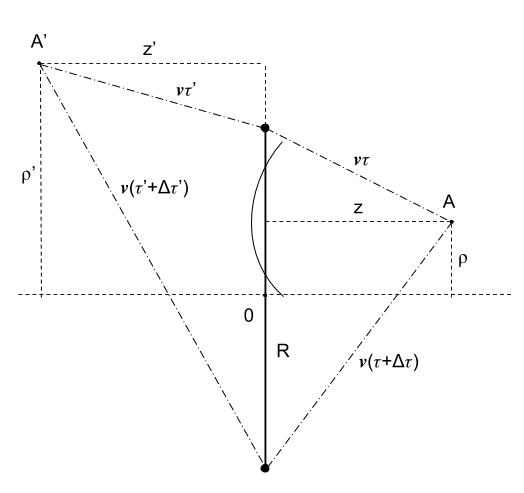
\includegraphics[scale=0.45]{PartialRadiation}
\caption{Фізичний зміст областей випромінювання} \label{fig:part_rad}
\end{center} \end{figure}

Область $ S_2 $ відповідає за події, коли частина крайніх точок джерела вже 
причинно пов'язана зі спостерігачем. Тобто частина джерела про яку вже відомо
спостерігачу (часоподібні), вже не має круглої форми та ще не охоплює 
всього джерела. В цій області спостерігається деякий перехідний процес в
якому значення перехідної функції поступово згасає на нуль.

Спостерігачі в області $ S_3 $ вже отримали всю інформацію про джерело. Для
них перехідний процес скінчено і зміни напруженості поля не спостерігається,
а отже напруженість електричного поля тут відсутня.

Для зони $ S_3 $ тільки $ E_x $ компонента електричного поля не дорівнює
нулю. Окрім того амплітуда $ E_x $ постійна для всіх подій з області $ S_3 $.

Також, аналізуючи геометрію процесу випромінювання на 
Рис.~\ref{fig:part_rad}, бачимо, що сигнал спостерігається з моменту 

\begin{equation} \begin{aligned} \label{eq:time1}
vt_1 = \begin{cases}
z, \rho < R \\
\sqrt{(\rho-R)^2+z^2}, \rho > R
\end{caes}.
\end{aligned} \end{equation}

Далі наступає момент початку області $ S_2 $, коли поле від найближчого 
краю диска досягає спостерігача:

\begin{equation} \begin{aligned} \label{eq:time2}
vt_2 = \sqrt{(\rho-R)^2+z^2} + \rho - \rho / R,
\end{aligned} \end{equation}

а закінчується область $ S_2 $ закінчується моментом, коли поле від 
найвіддаленішого краю диску досягає спостерігача:

\begin{equation} \begin{aligned} \label{eq:time3}
vt_3 = \sqrt{(\rho+R)^2+z^2}.
\end{aligned} \end{equation}

Перейдемо до магнітних складових перехідної функції плаского диску. Для 
отримання магнітних компонент поля скористаємось еволюційним коефіцієнтом 
\eqref{eq:imh}.

\textcolor{blue} { \begin{equation*} \begin{aligned}
\vect{H_\perp} = \frac{1}{\sqrt{\mu_0}} \left( 
\sum \limits_{m=-\infty}^{\infty} \int \limits_{0}^{\infty} d \nu
I_m^h \nabla_\perp \Psi_m + \sum \limits_{n=-\infty}^{\infty}
\int \limits_{0}^{\infty} d \chi I_n^e 
\crossprod{\vect{z_0}}{\nabla_\perp \Phi_n} \right)
\end{aligned} \end{equation*} }
%
\textcolor{blue} { \begin{equation*} \begin{aligned}
\nabla_\perp \Psi_m = e^{i m \varphi} \left( \vect{\rho_0} 
\sqrt{\nu} \frac{ J_{m-1}(\nu \rho) - J_{m+1}(\nu \rho) }{2} +
i m \vect{\varphi_0} \frac{J_m(\nu \rho)}{\sqrt{\nu} \rho} \right)
\end{aligned} \end{equation*} }
%
\textcolor{blue} { \begin{equation*} \begin{aligned}
\vect{H_\perp} = \frac{1}{\sqrt{\mu_0}} \left( 
\int \limits_{0}^{\infty} d \nu I_{-1}^h \nabla_\perp \Psi_{-1} +
\int \limits_{0}^{\infty} d \nu I_1^h \nabla_\perp \Psi_1 \right) = \\
= - \frac{A_0}{\sqrt{\mu_0}} \int \limits_{0}^{\infty} d \nu
\sqrt{\mu_0} \frac{iR}{4} J_1 (\nu R)
\frac{ U_0 [ W_-, Z ] - U_2 [ W_-, Z ] }{\sqrt{\nu}}  
e^{- i \varphi} \cdot \\ \cdot \left( \vect{\rho_0} 
\sqrt{\nu} \frac{ J_{2}(\nu \rho) - J_{0}(\nu \rho) }{2} +
i \vect{\varphi_0} \frac{J_1(\nu \rho)}{\sqrt{\nu} \rho} \right) -
\frac{A_0}{\sqrt{\mu_0}} \int \limits_{0}^{\infty} d \nu 
\sqrt{\mu_0} \frac{iR}{4} J_1 (\nu R) \cdot \\
\cdot \frac{ U_0 [ W_-, Z ] - U_2 [ W_-, Z ] }{\sqrt{\nu}} 
e^{i \varphi} \left( \vect{\rho_0} 
\sqrt{\nu} \frac{ J_{0}(\nu \rho) - J_{2}(\nu \rho) }{2} +
i \vect{\varphi_0} \frac{J_1(\nu \rho)}{\sqrt{\nu} \rho} \right)
\end{aligned} \end{equation*} }
%
\textcolor{blue} { \begin{equation*} \begin{aligned}
H_\varphi = \frac{R A_0}{4} 
\frac{e^{i \varphi} + e^{- i \varphi}}{\rho} \int \limits_{0}^{\infty} 
\frac{d\nu}{\nu} (U_0[ W_-, Z ] - U_2[ W_-, Z ]) J_1(\nu R) J_1(\nu \rho) = \\
= \frac{R}{2} \cos \varphi \int \limits_{0}^{\infty}
\frac{d\nu}{\nu \rho} (U_0[ W_-, Z ] - U_2[ W_-, Z ]) 
J_1(\nu R) J_1(\nu \rho)
\end{aligned} \end{equation*} }
%
\textcolor{blue} { \begin{equation*} \begin{aligned}
H_\rho = \frac{R A_0}{4} \frac{e^{i \varphi} - e^{- i \varphi}}{2i}
\int \limits_{0}^{\infty} d \nu (J_{0}(\nu \rho) - J_{2}(\nu \rho))
J_1(\nu R) (U_0[ W_-, Z ] - U_2[ W_-, Z ]) = \\
= \frac{R}{2} \sin \varphi \int \limits_{0}^{\infty} d \nu 
(J_0(\nu \rho) - \frac{J_1(\nu \rho)}{\nu \rho})
J_1(\nu R) (U_0[ W_-, Z ] - U_2[ W_-, Z ]) = \\
\end{aligned} \end{equation*} }
%
\textcolor{blue} { \begin{equation*} \begin{aligned}
\vect{H_\perp} \left( r, t \right) = \frac{A_0}{2} \left( 
\vect{\rho_0} \left( I_4 - I_3 \right) \sin \varphi +
\vect{\varphi_0} I_3 \cos \varphi  \right)
\end{aligned} \end{equation*} }
%
\textcolor{blue} { \begin{equation*} \begin{aligned}
H_z (r,t) = \frac{1}{\sqrt{\mu_0}} \sum \limits_{m=-\infty}^{\infty}
\int \limits_0^\infty \nu^2 d \nu h_m \Psi_m
\end{aligned} \end{equation*} }
%
\textcolor{blue} { \begin{equation*} \begin{aligned}
\Psi_m (\nu) = \frac{J_m(\nu \rho)}{\sqrt{\nu}} e^{im \varphi} 
\end{aligned} \end{equation*} }
%
\textcolor{blue} { \begin{equation*} \begin{aligned}
H_z (r,t) = 
\frac{1}{\sqrt{\mu_0}} \int \limits_0^\infty \nu^2 d \nu h_{1} \Psi_{1} +
\frac{1}{\sqrt{\mu_0}} \int \limits_0^\infty \nu^2 d \nu h_{-1} \Psi_{-1}
\end{aligned} \end{equation*} }
%
\textcolor{blue} { \begin{equation*} \begin{aligned}
H_z (r,t) = R A_0 \frac{e^{im \varphi}-e^{-im \varphi}}{2} \int_0^\infty 
d \nu J_1(\nu \rho) J_1 (\nu R)
U_1 \left[ -i \nu (ct-z), \nu \sqrt{c^2t^2-z^2} \right]
\end{aligned} \end{equation*} }
%
\textcolor{blue} { \begin{equation*} \begin{aligned}
H_z (r,t) = - R A_0 \sin \varphi \int_0^\infty 
d \nu J_1(\nu \rho) J_1 (\nu R) U_1 [ W_-, Z ] = \\
= - i R A_0 \sin \varphi \int_{0}^{\infty} J_1 \left( \nu R \right)
J_1 \left( \nu \rho \right) U_1 [ W_-, Z ]
\end{aligned} \end{equation*} }
%
\textcolor{blue} { \begin{equation*} \begin{aligned}
H_z \left( r, t \right) = - A_0 I_5 \sin \varphi
\end{aligned} \end{equation*} }
%
\begin{equation} \label{eq:linear_h_cyl}
\vect{H} (r, t) = \frac{A_0}{2} \Big( 
\vect{\rho_0} \left( I_4 - I_3 \right) \sin \varphi +
\vect{\varphi_0} I_3 \cos \varphi -
\vect{z_0} I_5 \sin \varphi \Big),
\end{equation}
%
де 
%
\begin{equation*}
I_3 = R \int \limits_{0}^{\infty}
\frac{d\nu}{\nu \rho} J_1(\nu R) J_1(\nu \rho)
\Big( U_0[ W, Z ] - U_2[ W, Z ] \Big),
\end{equation*}
%
\begin{equation*}
I_4 = R \int \limits_{0}^{\infty} d\nu J_1(\nu R) J_0(\nu \rho)
\Big( U_0[ W, Z ] - U_2[ W, Z ] \Big),
\end{equation*}
%
\begin{equation*}
I_5 = i R \int \limits_0^\infty 
d \nu J_1(\nu \rho) J_1 (\nu R)
U_1 \left[ -i \nu \left( \frac{ct}{\sqrt{\epsilon \mu}} - z \right), 
\nu \sqrt{\frac{c^2t^2}{\epsilon \mu}-z^2} \right].
\end{equation*}

В Декартовому базисі вектор напруженості магнітного поля матиме вигляд

\begin{equation} \begin{aligned} \label{eq:Hxyz}
\left( \begin{array}{c} H_x \\ H_y \\ H_z \end{array} \right) = 
\frac{A_0}{2} \left( \begin{array}{c}
- I_4 \sin \varphi \cos \varphi \\
I_3 \cos^2 \varphi + (I_4 - I_3) \sin^2 \varphi \\
- I_5 sin \varphi
\end{array} \right).
\end{aligned} \end{equation}

Для інтегралів $ I_3, I_4, I_5 $ аналітичні розв'язки, які представлено в 
додатку \ref{ch:lommel}, вдалось знайти лише на осі випромінювання 
($ \rho = 0 $). Відзначимо, що всі інтеграли мають дійсні значення, що витікає
з властивостей функції Ломмеля. Застосовуючи визначення функції Ломеля для  
виразу \eqref{eq:linear_h_cyl} на великій відстані від джерела, де плаский 
диск можна розглядати, як матеріальну точку, тобто $ z \gg R $ помічаємо, що 

\begin{equation*}
U_0[ W, Z ] - U_2[ W, Z ] = 
J_0 \left( \nu \sqrt{\frac{c^2t^2}{\epsilon \mu}  - z^2} \right),
\end{equation*}
%
тоді ортогональні поперечні компоненти електромагнітного поля попарно 
пропорційні через значення імпедансу вільного простору, в якому 
розповсюджується хвиля

\begin{equation} \label{eq:e2h}
\frac{E_x}{H_y} = \frac{E_y}{H_x} = 
\sqrt{\frac{\mu_0 \mu}{\epsilon_0 \epsilon}},
\end{equation}
%
що відповідає властивостям пласкої хвилі, а також підтверджує можливість 
апроксимації антен імпульсного випромінювання фізичною моделлю плаского 
стороннього електричного струму. Такий висновку можна дійти з того, що
саме пласку хвилю очікується побачити після випрямлення сферичного фронту
від ТЕМ рупора в плаский гіперболічною, або видовженою сферичною лінзою.

Звертаючись до аналітики з додатку \ref{ch:lommel} також помічаємо, що 
рівність \eqref{eq:e2h} також строго виконується і поблизу апертури, для 
всієї тривалості перехідного процесу. Рівність не виконується лише для 
області $ S_3 $, де $ \vect{E} = 0 $, а $ \vect{H}_\perp = const $.

%%%%%%%%%%%%%%%%%%%%%%%%%%%%%%%%%%%%%%%%%%%%%%%%%%%%%%%%%%%%%%%%%%%%%%%%%%%%%%%
\section{Властивості перехідної функції плаского диску}

Перехідною функцією антени називається електромагнітне випромінювання, 
збуджене нею, при часовій залежності сигналу у вигляді функції Хевісайда
\cite{imp:Kharkevich1950}. Перехідна функція дозволяє отримати 
випромінювання антени при збуджені сигналом довільної форми, не 
розв'язуючи задачу випромінювання, а користуючись принципом суперпозиції.

Знаючи момент приходу сигналу \eqref{eq:time1} та момент \eqref{eq:time3}
коли перехідна функція закінчиться, можна визначити тривалість
сигналу, збудженого струмом довільної форми $ f(t) $ та ефективною 
тривалістю $ \tau_0 $:

\begin{equation} \label{eq:e2h}
\frac{c \tau}{\sqrt{\epsilon \mu}} = \frac{c \tau_0}{\sqrt{\epsilon \mu}} + 
\sqrt{(\rho+R)^2 + z^2} - \begin{cases} z, \rho < R \\ 
\sqrt{(\rho-R)^2 + z^2}, \rho > R \end{cases},
\end{equation}
%
а отже тривалість електромагнітного імпульсу $ \tau $ пропорційна до 
$ \sqrt{\epsilon \mu} $.

Область визначення отриманої перехідної функції складається з трьох частин, 
які гарно проілюстровані залежністю $ E_x $ від часу та $ \rho $ при 
фіксованому значенні $ z $ (Рис.~\ref{fig:emp_rho}).
 
\begin{figure}[h] \begin{center}
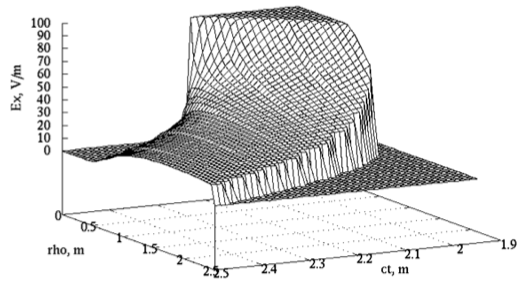
\includegraphics[scale=1.6]{MissileEffect}
\caption{Ефект електромагнітного снаряду ($ z = 2 $ м)} \label{fig:emp_rho}
\end{center} \end{figure}

На Рис.~\ref{fig:emp_rho} область $ S_1 $ зі сталим не нульовим значенням 
$ E_x $ компоненти поля спостерігаються лише для $ \rho < R $. За нею у 
часі наступає область $ S_2 $, де напруженість поля $ E_x $ поступово спадає 
на нуль. В області $ S_3 $ спостерігається $ E_x = 0 $.

Амплітуди всіх компонентів поля в області $ S_1 $ сталі, які можна отримати
з \eqref{eq:Exyz} та \eqref{eq:Hxyz} при $ \rho = 0 $:

\begin{equation*} \begin{aligned}
\vect{E} \{ S_1 \} = 
\vect{x_0} \frac{A_0}{4} 
\sqrt{\frac{\mu_0 \mu}{\epsilon_0 \epsilon}};
\end{aligned} \end{equation*}

\begin{equation*} \begin{aligned}
\vect{H} \{ S_1 \} = \vect{y_0} \frac{A_0}{4}.
\end{aligned} \end{equation*}

Цей ефект ближньої зони відомий під назвою електромагнітний снаряд і
зустрічається в багатьох роботах Содіна \cite{imp:Sodin1991, 
imp:Sodin1992-5, imp:Sodin1992-10, imp:Sodin1997}, роботах Ву 
\cite{imp:Wu1985, imp:Wu1987, imp:Wu1991}, в роботах Думіна
\cite{imp:Dumin1996} та в роботі Самсонова \cite{imp:Samsonov1986} але 
саме аналітичне значення амплітуди записано в перше, що є важливим для 
дослідження сильних полів.

Перехідна функція отримана без спрощень геометричної оптики, а отже 
справедлива для всіх точок спостереження ближньої зони. Отриманий результат 
дає змогу побачити форму електромагнітного імпульсу в залежності від 
азимутального кута при деякому $ z $ та $ \rho $, що лежать в ближній зоні.

З виразів для інтенсивності поля \eqref{eq:Exyz} та \eqref{eq:Hxyz} бачимо
центральну симетрію випромінювання відносно осі $ oZ $ для поперечних 
компонентів поля, отже достатньо дослідити лише залежність першій чверті.

\begin{figure}[h] \begin{center}
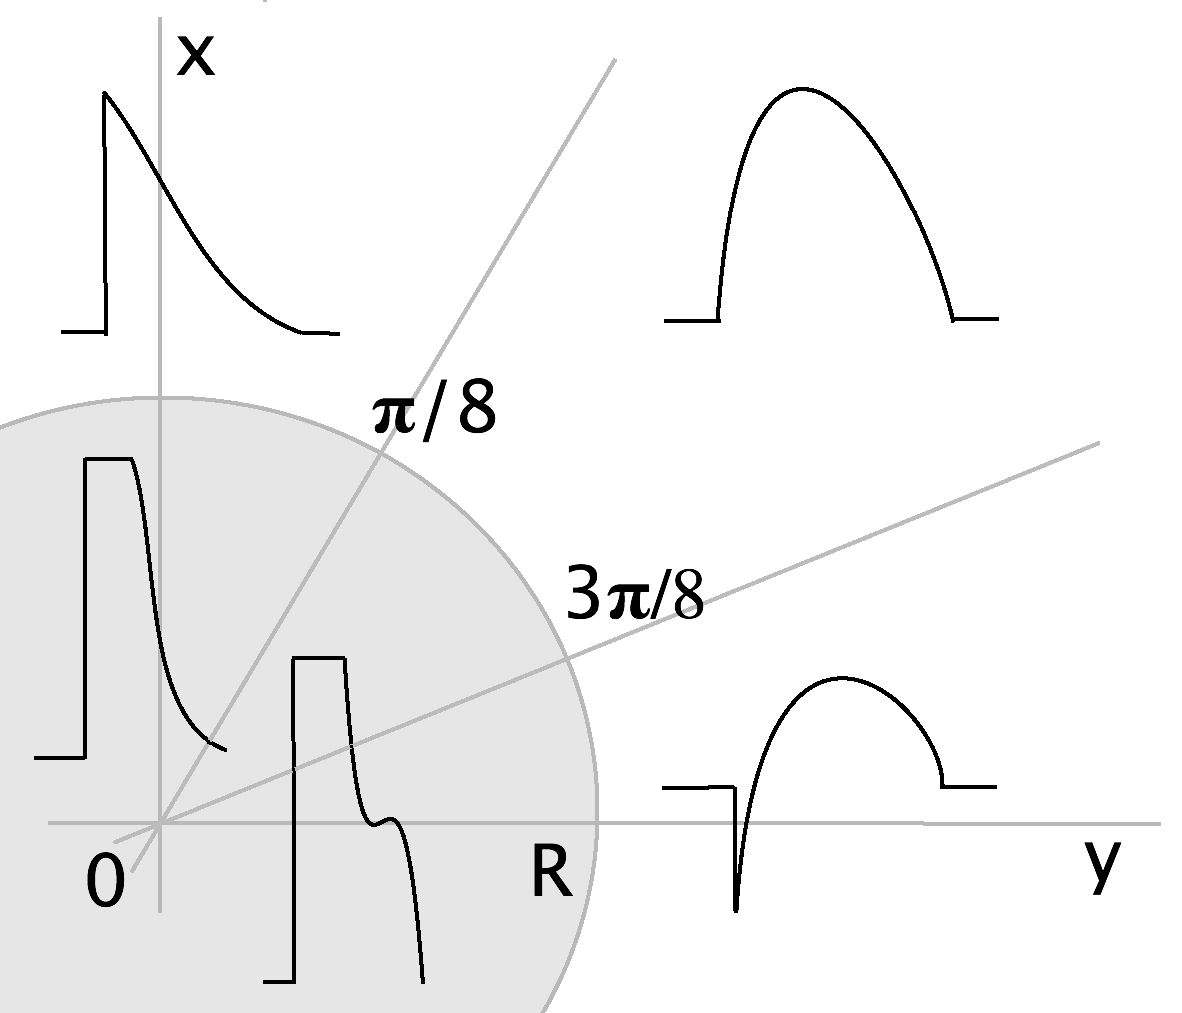
\includegraphics[scale=0.7]{LinearPulsShape}
\caption{Кутова залежність форми імпульсу ($ \rho = R/2 .. 2R $ м)} 
\label{fig:emp_shape}
\end{center} \end{figure}

На Рис.~\ref{fig:emp_shape} зображено залежність форми випроміненого 
імпульсу в залежності від кута спостереження в безпосередній близькості 
до джерела. Тут спостерігається ефект ближньої зони 
\textcolor{red}{[ПОСИЛАННЯ]}, де форма імпульсу залежить від напрямку 
розповсюдження і від відстані. З рисунку бачимо, що форма імпульсу в 
кожному напрямку в межах одного періоду симетрії унікальна, що можна 
використовувати в радарних та телекомунікаційних задачах 
(Дивись розділ~\ref{ch:neuron}).

За визначенням функції Ломмеля інтеграли $ I_3 $ та $ I_4 $ є 
нескінченною сумою інтегралів по трьом функціям Бесселя 
(\eqref{eq:i3_pol_int}, \eqref{eq:i4_pol_int}). При аналізі магнітного 
поля на осі випромінювання помічаємо, що поперечне магнітне поле для 
області $ S_1 $ пропорційне по значенням з компонентами 
електричного. Для області $ S_3 $ поперечне магнітне поле описується 
рядом з поліномів Лягера \eqref{eq:i3onaxis}.

\begin{figure}[h] \begin{center}
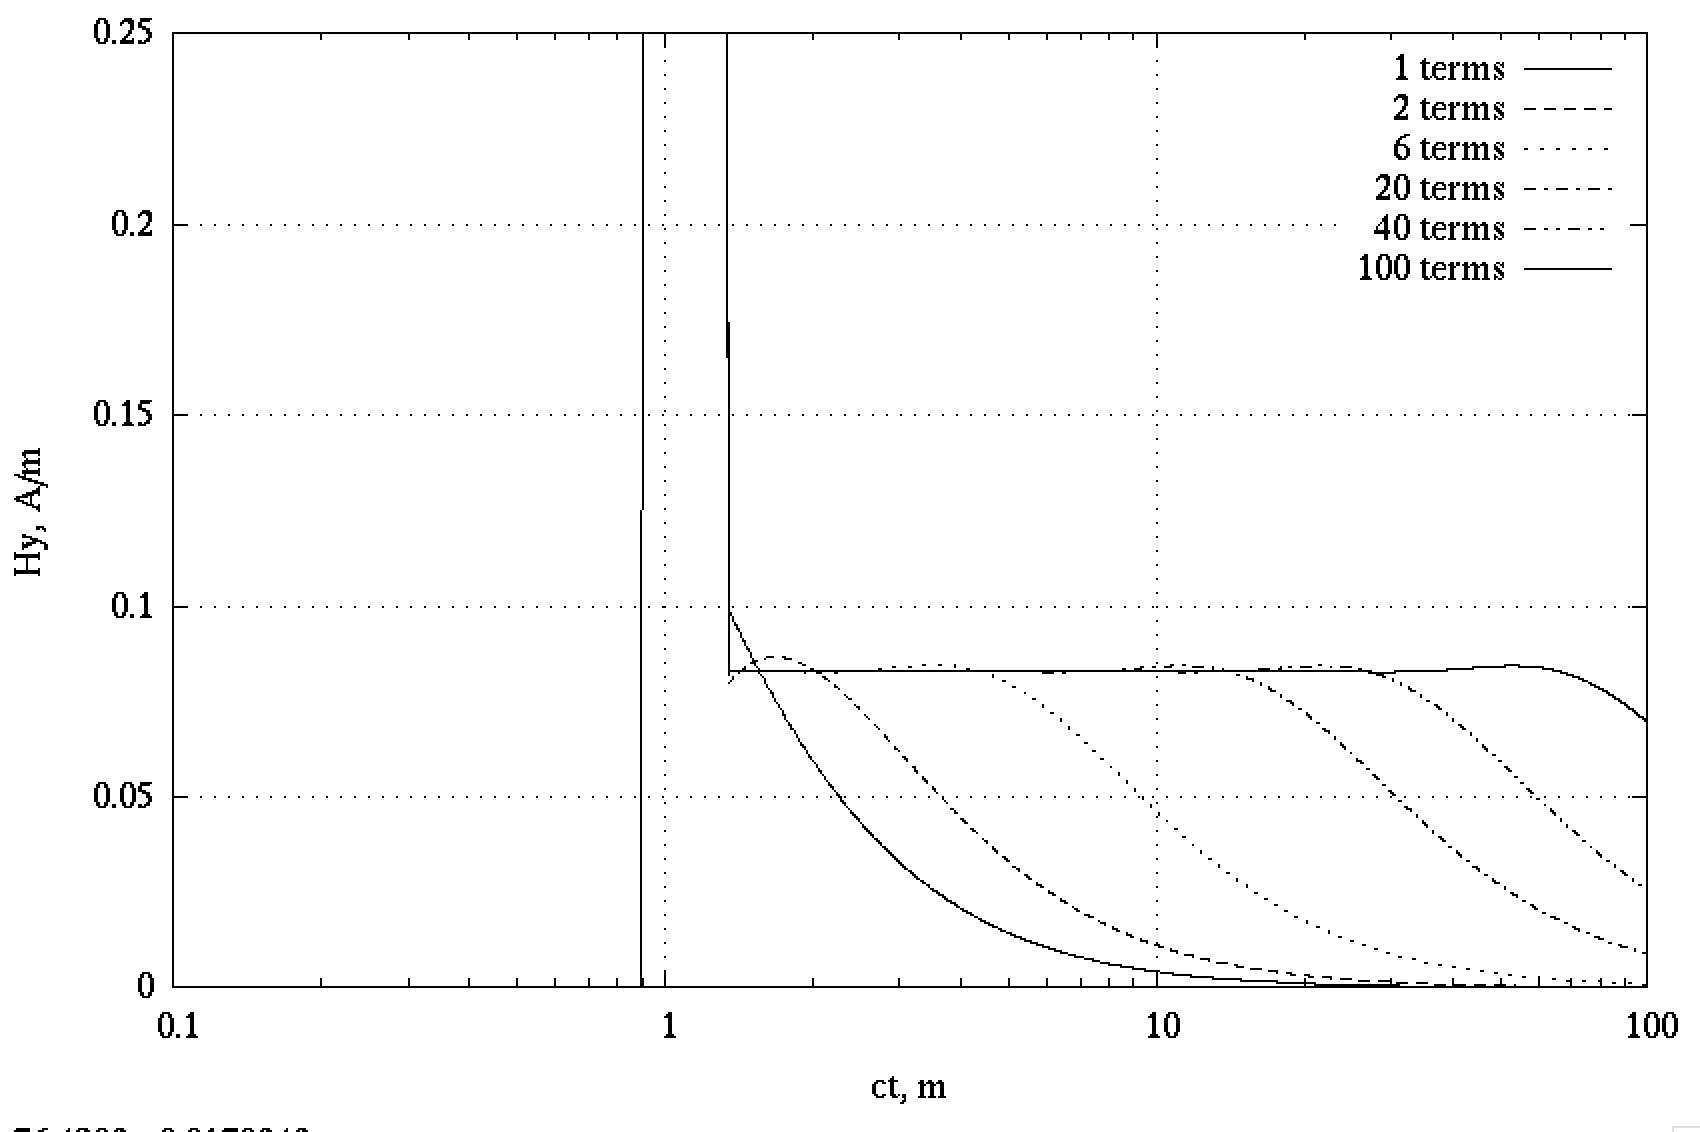
\includegraphics[scale=0.5]{SingulatiyFactorization}
\caption{Розклад сингулярності джерела} \label{fig:singulatiy_factorization}
\end{center} \end{figure}

На Рис.~\ref{fig:singulatiy_factorization} відображено процес сходження 
магнітної компоненти поля $ H_y $ при врахуванні різної кількості доданків
нескінченного поліному \eqref{eq:i3onaxis}. Бачимо, що з закінченням 
перехідного процесу наступає стаціонарне магнітне поле. Аналітично отриманий 
ряд сходиться дуже повільно - можемо зробити висновок, що модовий базис 
погано підходить для опису стаціонарних процесів, але доданки вищих порядків 
мають значний вклад лише при пропорційно великому часі спостереження.
Тобто, доданок $ m $ має внесок у значення функції $ H_z $ при $ ctm $.
Отже на Рис.~\ref{fig:emp_h_z}, можемо оцінити згасання амплітуди 
магнітостатики з відстанню від джерела. На Рис.~\ref{fig:emp_h_z} 
спостерігається \textcolor{red}{майже квадратичне} згасання статичної 
компонента з відстанню по $ z $. 

\begin{figure}[h] \begin{center}
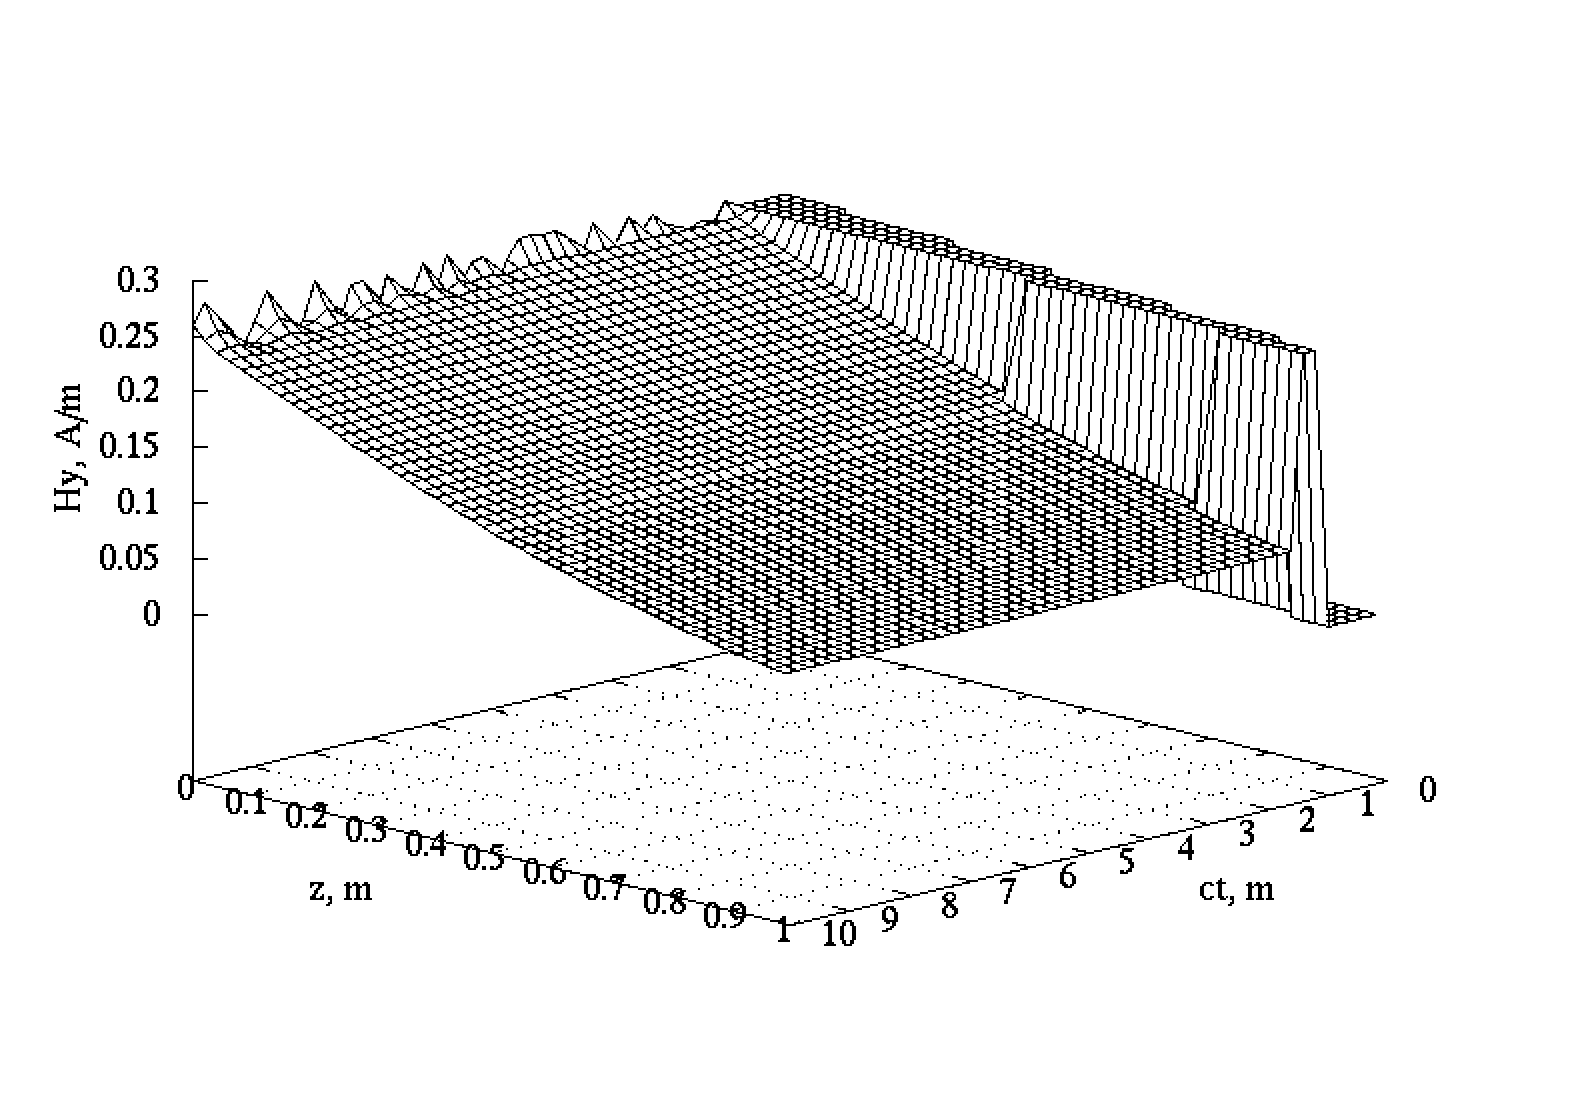
\includegraphics[scale=0.6]{StaticOnAxis}
\caption{Магнітностатичне поле ($ \rho = 0 $ м)} \label{fig:emp_h_z}
\end{center} \end{figure}

Розрахунок магнітних компонентів чисельно - розрахунок нескінченного 
поліному поліному від невласних інтегралів з повільним сходженням, що
хоча і наближено, але дає змогу оцінити розподіл магнітостатики в 
залежності від віддаленням від джерела. З Рис.~\ref{fig:emp_h_z} також 
помічаємо погане сходження поліному Лягера близько до сингулярності, тому 
результати чисельного розрахунку там не аналізуємо.

\begin{figure}[h] \begin{center}
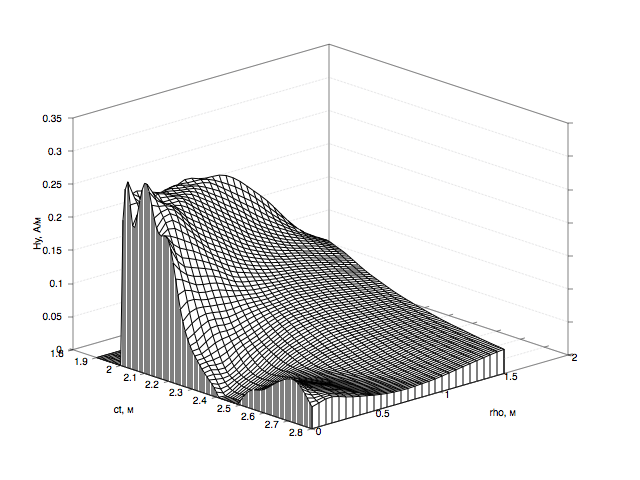
\includegraphics[scale=0.7]{LinearMagnetic}
\caption{Магнітностатичне поле ($ z = 2 $ м)} \label{fig:emp_h_rho}
\end{center} \end{figure}

На Рис.~\ref{fig:emp_h_rho} зображено залежність $ H_y (ct,\rho) $ при 
$ z = 2R $. Знову спостерігаємо поступове згасання амплітуди 
магнітооптичного з відстанню.

Розглянемо поведінку поздовжньої магнітної компоненти $ H_z $. З 
Рис.~\ref{fig:part_rad} та з аналітичних розв'язків для 
$ I_1, I_2, I_3, I_4 $ видно, що в області $ S_1 $, тобто коли 
спостерігач дізнався про наявність джерела, але за рахунок його форми
спостерігається один і то самий розподіл струму - плаский диск, ще 
невідомого спостерігачу радіусу. Відсутність нової інформації про 
джерело пояснює сталі значення відомих компонентів поля та дозволяє
зробити висновок про стале значення для компоненти $ H_z $ аж до 
моменту, коли найближчий край джерела та спостерігач не стануть 
причинно пов'язані.

Для всіх значень $ z \in \left[ \sqrt{c^2t^2-R^2}; R  \right] $ при 
$ \rho = 0 $ спостерігатися область $ S_1 $, а отже визначивши значення 
компоненти поля на осі випромінювання визначимо її сталу амплітуду
по всій області $ S_1 $. Таким чином, через залежність 
$ J_1 (\nu \rho) $ інтеграл $ I_5 $ на області визначення $ S_1 $ 
дорівнює нулю.

\begin{figure}[h] \begin{center}
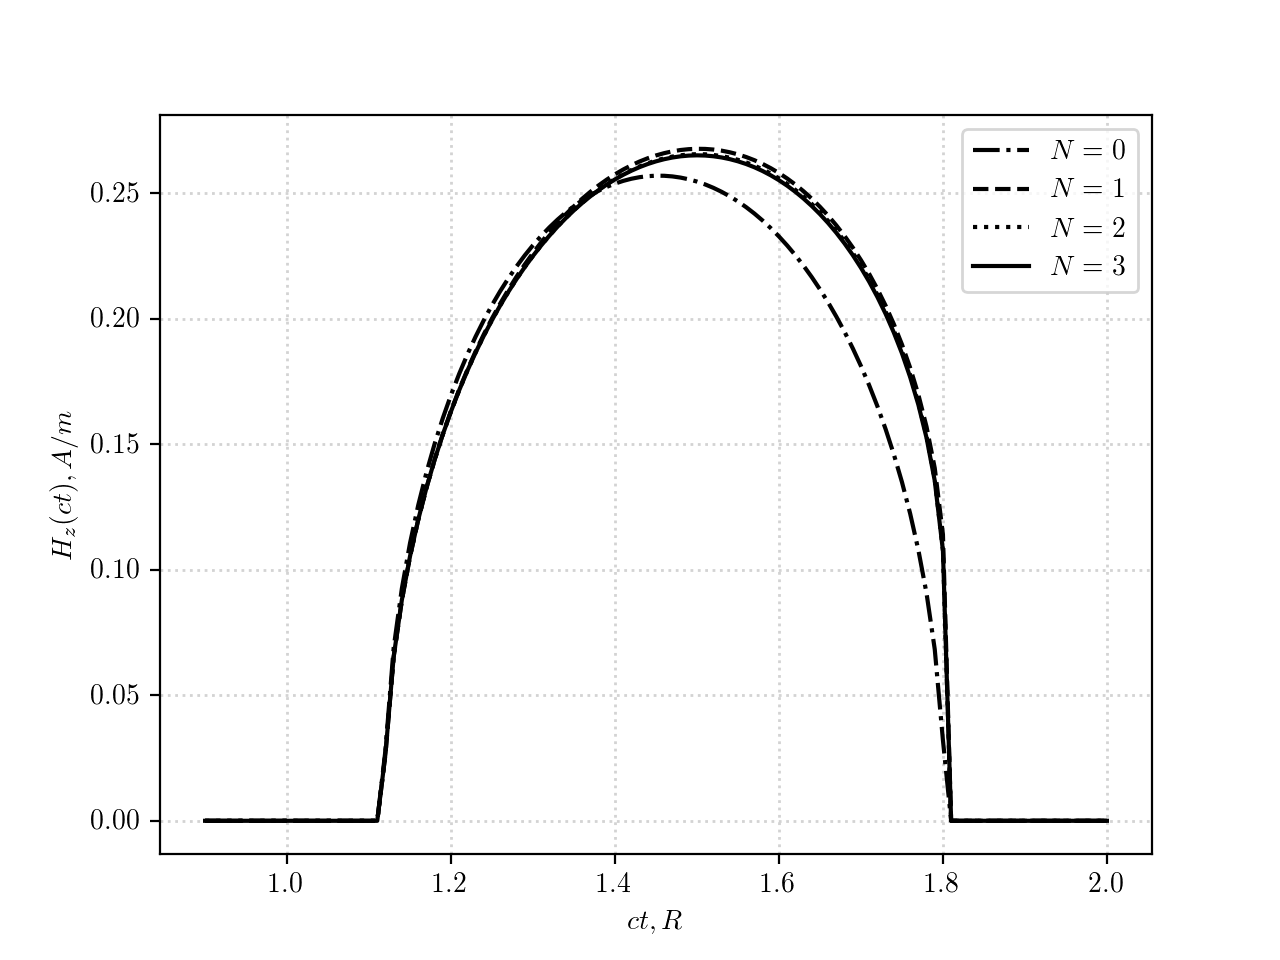
\includegraphics[scale=0.9]{Hz_terms}
\caption{$H_z$ в ($\rho = R/2$, $\varphi = -\pi/2$, $z = R$) при 
різній кількості доданків $ N $} \label{fig:hz_terms}
\end{center} \end{figure}

На Рис.~\ref{fig:hz_terms} проілюстровано вплив кількості врахованих 
доданків \eqref{eq:i5series} на форму компоненти $ H_z $. Помічаємо, що 
після двох врахованих доданків відхилення непомітне оку. Малий вплив 
доданків вищих порядків пояснюється тим, що поперечний базис методу 
еволюційних рівнянь гарно підходить для опису нестаціонарних процесів.

Розглянемо співвідношення продільної магнітної компоненти $ H_z $ та 
поперечної електричної компоненти $ E_x $. На Рис.~\ref{fig:ex_vs_hz}
бачимо, що компонента $ H_z $ починається з затримною. Плаский диск 
струму є апроксимацією ТЕМ джерела, а у вільному просторі поздовжня 
компонента повинна існувати, таким чином затримку поздовжньої 
компоненти можна розуміти, як трансформацію ТЕМ хвилі в ТЕ з прином 
часу в прожекторній зоні. Таким чином ефект електромагнітного снаряду 
можна трактувати, як процес формування хвилі у вільному просторі з TEM 
хвилі у рупорі.

\begin{figure}[h] \begin{center}
\includegraphics[scale=0.9]{Ex_vs_Hz}
\caption{$E_x$ і $H_z$ в ($\rho = R/2$, $\varphi = -\pi/2$, $z = R$)} 
\label{fig:ex_vs_hz}
\end{center} \end{figure}

В роботах Фарадея \textcolor{red}{[Фарадей]} зустрічається твердження, що 
випромінює не антена, а простір довкола неї. Саме це і спостерігається в 
області електромагнітного снаряду - через відсутність причинного зв'язку з 
краєм рупора, хвиля знаходячись у вільному просторі, має властивості хвилі у 
ТЕМ хвилеводі. Тобто, протягом тривалості електромагнітного сняряду ми 
спостерігаємо перетворення хвилі у хвилеводі на хвилю у вільному просторі, 
яка не може існувати без поздовжньої компоненти ($ H_z \neq 0 $) 
\textcolor{red}{[Борісов],[Хармут]}. Також відмітемо, що форма часової 
залежності не впливає на затримку у появі $ H_z $ компоненти поля - вона 
залежить лише від наявності зони апертури антени з рівним часовим фронтом 
та спостеріратиметься в усіх точках прочтору, що знаходиться на нормалі до 
цієї "пласкої" частини фронту в апертурі.

Таким чином, можемо узагальнити твердження Фарадея для нестаціонарного 
процесу: розповсюдження хвилі у вільному просторі, почнеться тільки тоді, 
коли спостерігач дізнається про те, що розподіл струму в апертурі просторово
змінюється, а до цього, спостерігається той самий процес, що і у 
внутрішньому просторі антени. \textcolor{red}{Для реальних джерел...}

Також, узагальнемо фізичний смисл областей випромінювання: $ S_1 $ -
область формування хвилі у вільному просторі, $ S_2 $ - область 
несталого (перехідного) процесу випромінювання, $ S_3 $ - область
усталеного процесу.

%%%%%%%%%%%%%%%%%%%%%%%%%%%%%%%%%%%%%%%%%%%%%%%%%%%%%%%%%%%%%%%%%%%%%%%%%%%%%%
\section{Збуджувальний імпульс довільної форми}

Оцінимо вплив ефектів ближньої зони на поле, що породжене пласким диском 
електричного струму на прямокутний збуджувальний імпульс тривалістю 
$ \tau_0 $, тобто вмикання струму до амплітуди $ A_0 $ Вольт і послідовне 
його вимкнення з затримкою $ \tau_0 $ секунд:

\begin{equation}
\vect{j} (r,t) = \vect{j_0} (r,t) - \vect{j_0} (r,t-\tau_0),
\end{equation}

де $ \vect{j_0} $ - струм, що породжує електричну $ \vect{E_0} $ і магнітну 
$ \vect{H_0} $ перехідні функції. Таким чином, користуючись принципом 
суперпозиції

\begin{equation}
\vect{E} (r,t) = \vect{E_0} (r,t) - \vect{E_0} (r,t-\tau_0).
\end{equation}

Тривалість перехідної функції $ \vect{E_0} $ на осі випромінювання 
$ \sqrt{z^2+R^2} - z $, а її максимальне значення досягається при малих 
відствнях та наближається до $ R $. Тому, якщо затримка перед вимкненням 
струму $ c \tau_0 $ триваліша за $ R $ ефект накладання на осі не 
спостерігається. Якщо, також, врахувати $ \rho \neq 0 $ можна отримати 
$ c \tau_0 > 2R $.

Користуючись методикою інтегрування Дюамеля,
\cite[ст. 40]{imp:Kharkevich1950} знайдемо поле, від антени з відомою 
перехідною функцією $ \vect{E_0} (r,t) $ та $ \vect{H_0} (r,t) $ збудженою 
сигналом плавної форми $ f(t) $ з максимальною амплітудою $ A_0 $ В:

\begin{equation} \label{eq:duhamel}
\vect{E} = \int_0^t \derivat{f}{\tau} \vect{E_0} (t - \tau) d \tau.
\end{equation}

Інтеграл \eqref{eq:duhamel} є узагальненням принципу суперпозиції, а отже
працюватиме лише для лінійної залежності електаричної індукції від 
напруженості поля. Проте, його використання доцільне для вивчення 
напруженості імпульсного поля, яка при накладанні може викликати 
необхідність врахування нелінійних ефектів накшталт пробою в сильних полях.

Розглянемо в якості форми збудження плавне наростання амплітуди струму до 
значення $ A_0 $ протягом $ \tau_0 $ за метрикою 1-99 risetime у вигляді 
сигмоїдальної функції.

\begin{figure}[h] \begin{center}
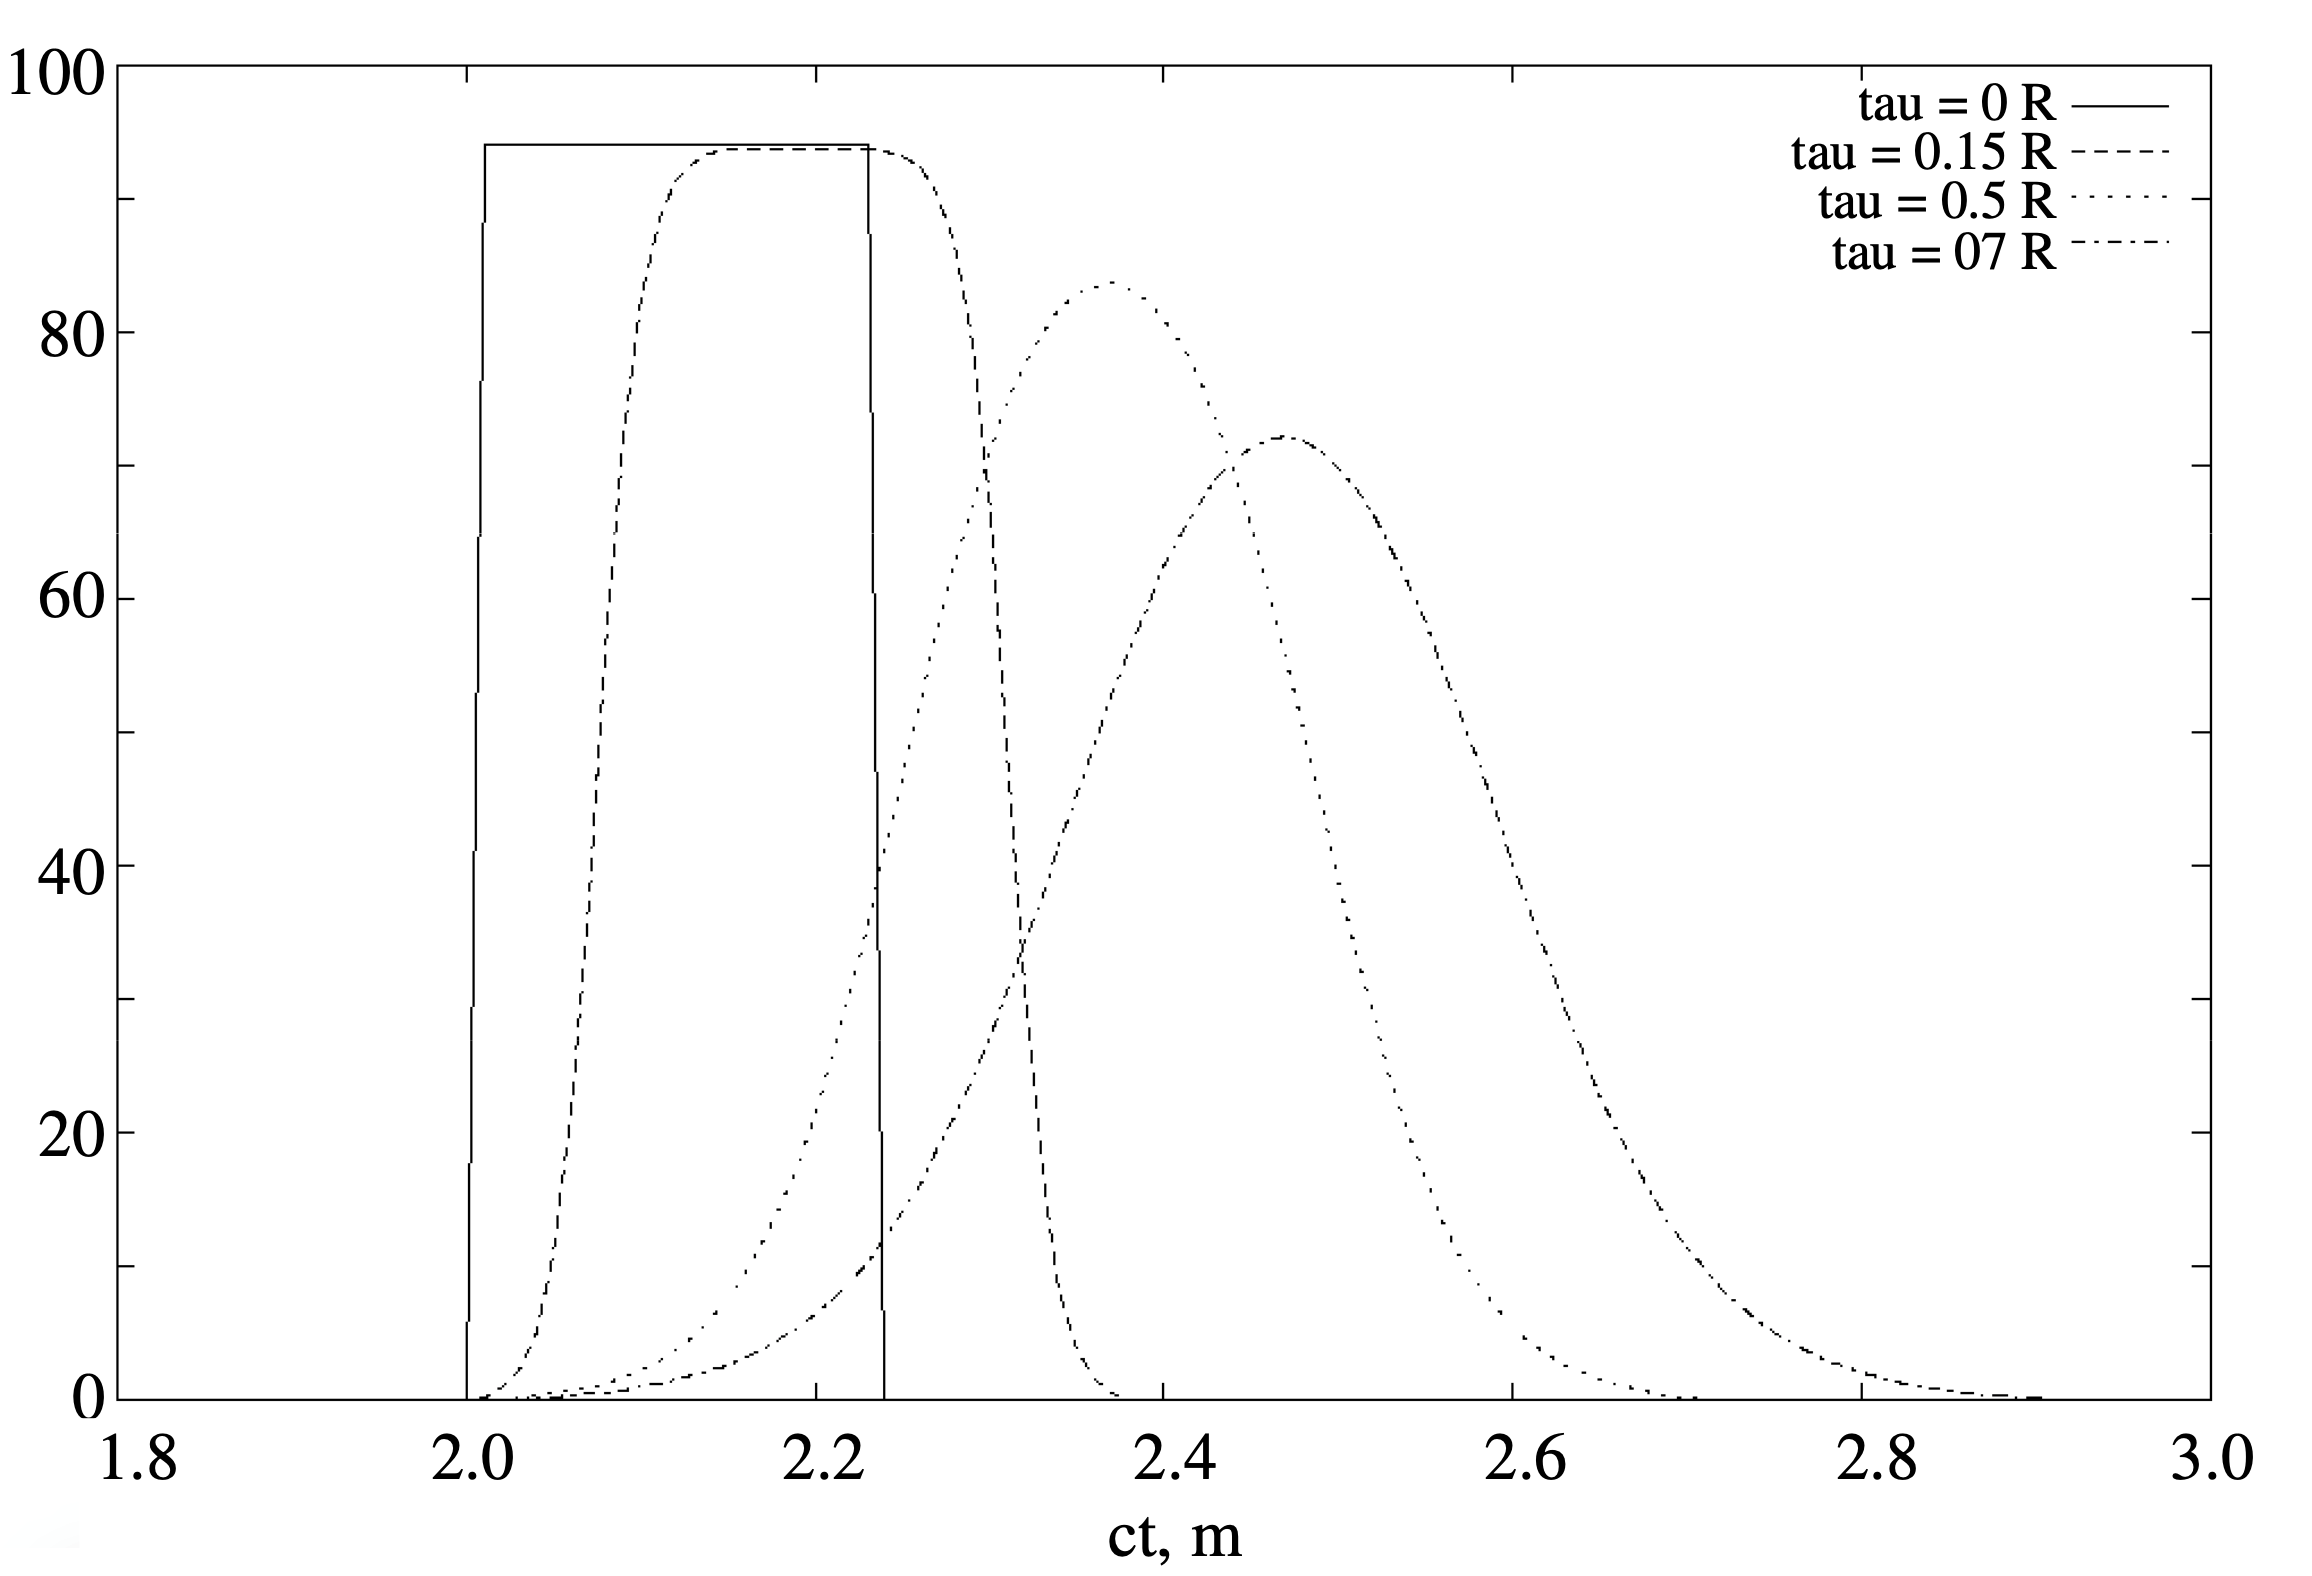
\includegraphics[scale=0.4]{Sigmoidal}
\caption{$ E_x $ компонента поля від сигмоїдального збудження}
\label{fig:ex_sigmoidal}
\end{center} \end{figure}

Результати представлені на Рис.~\ref{fig:ex_sigmoidal} сходяться з 
експериментальними дослідженнями отримані незалежно Баумом та Ву.

Тепер розглянемо збуджувальний сигнал у вигляді $ f(t) = \sinc t $.
Така часова залежність збудження для плаского диску породжує імпульсне
швидко-осцилююче поле. Розглянемо інтерференцію цього поля в ближній зоні.
На Рис.~\ref{fig:ex_sinc} зображено залежність напруженості електричного 
поля $ E_x $ від часу для двох точок спостереження.

\begin{figure}[h] \begin{center}
\includegraphics[scale=0.9]{ex_sinc}
\caption{$ E_x $ компонента поля від $ \sinc t $ збудження}
\label{fig:ex_sinc}
\end{center} \end{figure}

З Рис.~\ref{fig:ex_sinc} бачимо, що на більшому віддалені від джерела, 
максимальна напруженість поля більша за максимальну напруженість, що була 
досягнута при менших відстанях. При накладанні перехідних функцій початку 
збудження та дзеркального його продовження спостерігається протифазне 
накладання, що з відстанню переходе у синфазне і амплітуда сигналу 
збільшується в межах $ 20\% $. Таким чином при роботі з сильними 
швидко-асцилюючими імпульсними полями цей ефект треба враховувати щоб 
уникнути електричного пробою в межах короткотривалих піках напруженості.

%%%%%%%%%%%%%%%%%%%%%%%%%%%%%%%%%%%%%%%%%%%%%%%%%%%%%%%%%%%%%%%%%%%%%%%%%%%%%%%
\section{Врахування краєвих ефектів випромінювання}

\textcolor{red}{Шматько Александр Александрович на защите Лены Овсянниковой 
замечал что, для того чтоб задачу можно было назвать апертурной, нужно учеть 
в модели краевое излечение}
